\documentclass[10pt,a4paper,twocolumn]{article}

\usepackage[utf8]{inputenc}
\usepackage[T1]{fontenc}
\usepackage[spanish,es-nodecimaldot]{babel}
\usepackage{lmodern}
\usepackage{microtype}
\usepackage{amsmath}
\usepackage{amssymb}
\usepackage{geometry}
\usepackage{booktabs}
\usepackage{tabularx}
\usepackage{array}
\usepackage{enumitem}
\usepackage{siunitx}
\usepackage{graphicx}
\usepackage{float}
\usepackage{dblfloatfix}
\usepackage[section]{placeins}
\usepackage{xcolor}
\usepackage{tikz}
\usetikzlibrary{arrows.meta,positioning,fit}
\usepackage[round,authoryear]{natbib}
\usepackage{hyperref}

\geometry{margin=2.5cm}
\setlength{\columnsep}{0.7cm}
\raggedbottom
\setlist[itemize]{itemsep=0.2em}
\sisetup{output-decimal-marker={,}}
\newcolumntype{Y}{>{\raggedright\arraybackslash}X}
\graphicspath{{figuras/}{../latex-historial/figuras/}{../latex-15p-review/figuras/transductores/}{../latex-15p-review/figuras/acondicionamiento/}{../latex-15p-review/figuras/excitacion/}{../latex-15p-review/figuras/interfaces/}{../../Urucom_2026_compact/imagenes/}{../../Propuesta Urucom/Imagenes/}}

\addto\captionsspanish{\renewcommand{\tablename}{Tabla}}
\hypersetup{colorlinks=true,linkcolor=black,citecolor=black,urlcolor=blue}

% Marco de figura pendiente: reserva el espacio real que ocupara la lamina.
% Al incorporar las figuras definitivas se reemplaza por \includegraphics.
\newcommand{\figpendiente}[2][0.42]{%
  \setlength{\fboxsep}{6pt}%
  \fbox{\parbox[c][#1\columnwidth][c]{\dimexpr\columnwidth-2\fboxsep-2\fboxrule\relax}{%
    \centering\footnotesize\itshape #2}}%
}

%\title{Diseño e implementación de un sistema electrónico multicanal del tipo IoT
%para caracterización geotécnica del suelo mediante ondas sísmicas}
\author{}
\date{}

\begin{document}

\twocolumn[
  \begin{center}
    {\LARGE\bfseries Diseño e implementación de un sistema electrónico
     multicanal del tipo IoT para caracterización geotécnica del suelo
     mediante ondas sísmicas\par}
    \vspace{0.9em}
    {\large\itshape Proyecto final de carrera -- Primera presentación\par}
    \vspace{1.1em}
    {\footnotesize
     \begin{tabular}{@{}ll@{\hspace{3em}}ll@{}}
       \textbf{Alumno:} & Elías David Álvarez Martínez &
       \textbf{Carrera:} & Ingeniería Electrónica.\\
       \textbf{Matrícula:} & Y24127 &
       \textbf{Tutor:} & Enrique A. Vargas Cabral, Ph.D.\\
     \end{tabular}\par}
    \vspace{1.8em}
  \end{center}
]

\section{Importancia de la caracterización geotécnica del suelo}

La respuesta de una obra civil frente a cargas estáticas y dinámicas depende de propiedades mecánicas del terreno que varían con la profundidad y, en general, también lateralmente. Reconocer esa variación (espesores, contactos, rellenos y zonas de menor rigidez) es una condición previa al dimensionamiento de fundaciones, a la evaluación de asentamientos y a la estimación de la respuesta sísmica de sitio.

Entre las magnitudes que describen ese comportamiento, la velocidad de propagación de las ondas de corte, $V_S$, ocupa un lugar particular porque se vincula de forma directa con la rigidez del medio a pequeñas deformaciones. Para un medio elástico de densidad $\rho$, el módulo de corte a pequeñas deformaciones queda determinado por

\begin{equation}
G_{\max}=\rho\,V_S^{2},
\end{equation}

de manera que medir $V_S$ equivale, conocida la densidad, a medir la rigidez del suelo en el rango de deformaciones en que su comportamiento puede considerarse aproximadamente elástico. Esa equivalencia explica por qué el perfil $V_S(z)$ se ha consolidado como parámetro de entrada en la clasificación sísmica de sitios y en el análisis de respuesta dinámica del terreno \citep{Kramer1996,Foti2014}.

Conviene fijar desde el inicio una precisión que condiciona todo lo que sigue: ninguna técnica de prospección entrega una imagen exacta del subsuelo, sino un modelo compatible con los datos, con la geometría del ensayo y con los supuestos de interpretación. Esa distinción determina qué información debe preservar el instrumento y hasta qué profundidad puede sostenerse una afirmación.

Se tiene como objetivo de este proyecto de fin de grado el diseño, la implementación y la evaluación experimental de un sistema electrónico multicanal del tipo IoT para la caracterización geotécnica del suelo mediante ondas sísmicas, orientado a profundidades de investigación de hasta 50 m. La contribución que se presenta en esta primera etapa es de instrumentación: la integración y la evaluación con datos reales de una cadena de medida completa, desde la fuente instrumentada y el geófono hasta el acondicionamiento analógico, la conversión analógico-digital, la temporización, el almacenamiento y el procesamiento que conduce a un perfil $V_S(z)$ preliminar. El interés de construirla en lugar de adquirirla no está en suponer que la industria carezca de soluciones, sino en disponer de una plataforma auditable en cada etapa, condición que el instrumental comercial cerrado no ofrece a un laboratorio universitario.

Conviene precisar el centro de gravedad del trabajo antes de continuar. Se trata de un proyecto de fin de grado de Ingeniería Electrónica, de modo que el objeto de diseño, implementación, caracterización y validación es el sistema de instrumentación. La caracterización geotécnica y el método MASW constituyen el contexto de aplicación: son los que definen los requerimientos que el instrumento debe satisfacer y el criterio con el que se juzga si los satisface. Las secciones 2 a 7 desarrollan en consecuencia únicamente la física necesaria para derivar esos requerimientos, y la interpretación geológica se mantiene en todo el documento dentro del límite estricto de verificar la plausibilidad de los resultados obtenidos.

Ese objetivo formal debe distinguirse con claridad del alcance efectivamente alcanzado hasta hoy, y el documento mantiene esa separación en todas sus secciones:

\begin{itemize}
\item \textbf{Objetivo de diseño.} Una plataforma multicanal orientada a investigar hasta 50 m de profundidad.
\item \textbf{Alcance demostrado con la campaña y la cadena actuales.} Adquisición, procesamiento e inversión con soporte de investigación del orden de 10 a 11 m.
\item \textbf{Brecha experimental.} Aumentar la energía coherente de baja frecuencia, completar el hardware multinodo y realizar las validaciones metrológicas y geofísicas independientes que todavía faltan.
\end{itemize}

Las secciones 2 a 7 establecen qué se desea medir y por qué mediante ondas superficiales; la sección 8 traduce esa elección en requerimientos cuantitativos; la sección 9 presenta el diseño electrónico como respuesta a ellos; las secciones 10 y 11 describen la validación y sus resultados, y la 12 delimita lo que aún no puede afirmarse.

\section{Métodos tradicionales de caracterización del suelo}

El reconocimiento geotécnico convencional se apoya en ensayos que establecen contacto físico con el terreno. El ensayo de penetración estándar (SPT) da una medida indirecta de resistencia y permite recuperar muestras a intervalos discretos, con la ventaja de una práctica extendida y correlaciones documentadas; el ensayo de penetración con cono (CPT y su variante piezométrica CPTu) mejora la continuidad vertical del registro y reduce la dependencia del operador, aunque pierde aplicabilidad en gravas o niveles cementados.

Cuando el objetivo es directamente una velocidad sísmica, la referencia son los ensayos en pozo: el downhole registra en profundidad las llegadas generadas en superficie y el crosshole mide el tiempo de tránsito entre perforaciones vecinas, ofreciendo la mejor resolución vertical disponible para $V_S$. Ambos comparten la limitación que motiva este trabajo, ya que exigen perforar, con el costo y el plazo asociados, y describen el suelo sólo en el entorno del pozo.

De esa comparación se desprende la motivación de los métodos no invasivos. Una obra necesita reconocer la variación lateral de la rigidez en un volumen extenso, y un conjunto de sondeos puntuales resulta costoso de densificar. Los métodos basados en la propagación de ondas mecánicas desde la superficie permiten cubrir esa extensión sin perforar, a cambio de trabajar con una magnitud que se infiere en lugar de medirse por contacto. A ese argumento se agrega un campo de aplicación que el carácter no invasivo habilita de manera casi exclusiva: el control de calidad y el seguimiento de obras ya construidas. Una traza vial, un terraplén o una plataforma pueden recorrerse de forma repetida y sin daño para verificar la uniformidad de la compactación durante la construcción, y para detectar posteriormente la degradación o la pérdida de rigidez que anticipa la necesidad de mantenimiento. Un ensayo destructivo no admite esa repetición sobre la misma obra.

\section{Métodos basados en ondas mecánicas}

La caracterización sísmica se apoya en que las propiedades mecánicas del medio gobiernan cómo se propaga una perturbación, y en que esa propagación deja magnitudes observables en superficie: tiempos de llegada, amplitudes y relaciones de fase entre puntos separados. Medirlas permite estimar las propiedades sin acceder a la profundidad de interés.

Las familias de métodos se distinguen por qué observable explotan. La refracción sísmica utiliza los tiempos de primera llegada de ondas de cuerpo refractadas críticamente y resulta apropiada cuando la velocidad crece de manera monótona con la profundidad; su punto débil conocido es la incapacidad de detectar capas de baja velocidad ocultas bajo otras más rápidas. La reflexión aprovecha los contrastes de impedancia y alcanza mayor profundidad, pero requiere fuentes de energía considerable y una relación señal a ruido difícil de obtener en el rango somero. Los métodos de ondas superficiales, en cambio, explotan la dependencia de la velocidad de fase con la frecuencia, y esa dependencia es precisamente lo que codifica la variación de rigidez con la profundidad.

Para un ensayo desde superficie orientado a $V_S$ en los primeros metros, la última familia presenta una ventaja física decisiva. Un impacto vertical aplicado en la superficie de un semiespacio destina la mayor parte de la energía elástica radiada a la onda Rayleigh \citep{Foti2014}, cuya amplitud decae con la distancia de forma considerablemente más lenta que la de las ondas de cuerpo. El método aprovecha así la componente más energética del campo de ondas en lugar de combatirla como ruido, lo que resulta determinante cuando la fuente disponible es un impacto manual y no una fuente sísmica de gran porte.

\section{Fundamentos de propagación de ondas en un medio}

En un medio elástico, homogéneo e isótropo, la propagación de perturbaciones infinitesimales queda descrita por dos velocidades independientes, asociadas a los dos modos posibles de deformación. La velocidad de las ondas de compresión y la de las ondas de corte se expresan en función de los parámetros de Lamé $\lambda$ y $\mu$ y de la densidad $\rho$ como

\begin{equation}
V_P=\sqrt{\frac{\lambda+2\mu}{\rho}},
\qquad
V_S=\sqrt{\frac{\mu}{\rho}} .
\end{equation}

La segunda expresión es la que conecta la medición con el objetivo planteado en la sección 1: como $\mu$ coincide con el módulo de corte a pequeñas deformaciones, obtener $V_S$ equivale a obtener $G_{\max}$ salvo por el factor de densidad. Esa relación resulta especialmente conveniente porque las dos magnitudes involucradas tienen rangos de variación muy dispares. La densidad de los suelos habituales se mantiene aproximadamente entre 1,4 y 2,2 t/m³, es decir dentro de un factor menor que dos, mientras que $V_S$ recorre desde algunas decenas de metros por segundo en suelos blandos hasta varios cientos en materiales densos o cementados. Como $G_{\max}$ depende del cuadrado de la velocidad, su variación queda dominada por $V_S$, y un valor de densidad estimado con precisión moderada resulta suficiente para obtener una rigidez útil \citep{Kramer1996,Foti2014}. Las ondas de compresión, en cambio, resultan poco informativas en el rango somero saturado: por debajo del nivel freático $V_P$ queda gobernada por la compresibilidad del agua intersticial y tiende hacia unos 1500 m/s con independencia del estado del esqueleto sólido, de modo que pierde sensibilidad justamente a la propiedad que interesa medir \citep{Foti2014,Foti2018}.

Ambas velocidades quedan vinculadas por el coeficiente de Poisson,

\begin{equation}
\nu=\frac{V_P^{2}-2V_S^{2}}{2\left(V_P^{2}-V_S^{2}\right)},
\end{equation}

relación que conviene retener porque $\nu$ no fue medido en este trabajo y debió adoptarse por hipótesis en la inversión, con las consecuencias que se analizan en la sección 11.3.

Las expresiones anteriores suponen un medio homogéneo y perfectamente elástico, y conviene señalar que ninguna de las dos condiciones se cumple en el terreno real. El suelo es un medio estratificado, y esa estratificación no es una desviación molesta del modelo sino precisamente lo que el ensayo se propone reconstruir. El suelo tampoco es perfectamente elástico: disipa energía a medida que la onda avanza, por lo que la amplitud registrada en un receptor lejano se reduce tanto por divergencia geométrica como por atenuación material, y esta última crece con la frecuencia.

De ahí se sigue una consecuencia que condiciona el diseño del instrumento. Si la señal útil se debilita al aumentar la distancia y la frecuencia, entonces el margen entre señal y ruido de la cadena de medida deja de ser una cifra de mérito genérica y pasa a ser la variable que determina cuál es la máxima longitud de onda que todavía puede reconocerse y, por lo tanto, hasta qué profundidad puede investigarse.

\section{Ondas de cuerpo y ondas superficiales}

Las ondas de cuerpo se propagan por el volumen del medio y se distinguen por su polarización: la P desplaza las partículas en la dirección de propagación y la S lo hace transversalmente, razón por la cual es esta última la que involucra al módulo de corte. Dentro de la onda S conviene además distinguir dos polarizaciones, porque de ellas depende qué onda superficial puede formarse: la componente SV oscila en el plano vertical que contiene la dirección de propagación y la SH en el plano horizontal perpendicular a él.

Las ondas superficiales no son un tercer tipo de onda independiente, sino el resultado de la interacción de las anteriores con la superficie libre del terreno. Cuando una onda P y una onda SV inciden sobre esa frontera, la condición de tensión nula obliga a que se conviertan mutuamente al reflejarse, y para ciertas combinaciones de ángulo y frecuencia ambas quedan acopladas en una perturbación que no se propaga hacia el interior sino que viaja paralela a la superficie, con amplitud que decae exponencialmente con la profundidad. Esa perturbación es la onda Rayleigh: combina por construcción una componente vertical y una longitudinal, y describe en el semiespacio homogéneo un movimiento elíptico retrógrado. Su velocidad de fase se sitúa entre el 87 \% y el 96 \% de $V_S$ según el coeficiente de Poisson, lo que la convierte en un buen sustituto observable de la velocidad de corte.

La componente SH no puede acoplarse a la P por razones de polarización, y por eso no participa de la onda Rayleigh. Puede, en cambio, quedar atrapada por reflexiones múltiples dentro de una capa superficial de menor velocidad apoyada sobre un sustrato más rápido, y forma entonces la onda Love. Como su movimiento es horizontal y transversal, no produce señal apreciable en un geófono vertical; por esa razón la onda Love queda fuera del alcance de este trabajo, cuya cadena de medida registra únicamente la componente vertical.

La relación entre la Rayleigh y $V_S$ es la que convierte a la primera en un observable útil. Como la velocidad de fase Rayleigh es del orden del 90 \% de la velocidad de corte del material que la onda efectivamente muestrea, una medición de $c_R$ constituye una medición aproximada de $V_S$ una vez resuelto qué volumen del terreno correspondió a cada frecuencia.

Esa correspondencia entre frecuencia y volumen muestreado la fija la longitud de onda. Para una frecuencia $f$ y una velocidad de fase $c_R(f)$,

\begin{equation}
\lambda_R(f)=\frac{c_R(f)}{f},
\end{equation}

y el desplazamiento asociado a una onda Rayleigh decae con la profundidad en una escala comparable a $\lambda_R$. Las longitudes de onda cortas quedan por tanto controladas por el material somero, mientras que las largas integran un volumen mayor y alcanzan mayor profundidad. La regla práctica $z\approx\lambda/2$, en la que $z$ es la profundidad de investigación, entendida como la profundidad máxima hasta la cual la medición conserva sensibilidad apreciable, resume esa proporcionalidad y se emplea de forma habitual para estimar la profundidad de investigación de una campaña, pero no asigna una profundidad exacta a cada frecuencia: las funciones de sensibilidad son distribuidas y se superponen entre frecuencias vecinas. De ahí se sigue una advertencia que resulta decisiva al interpretar los registros: observar energía a una frecuencia baja no demuestra que exista allí una onda Rayleigh útil, criterio que la sección 12 desarrolla al discutir la fuente.

\section{Utilización de ondas superficiales para la caracterización de suelos}

En un medio homogéneo la velocidad Rayleigh no depende de la frecuencia. La dispersión aparece cuando el medio está estratificado, porque cada longitud de onda muestrea una combinación distinta de capas y se propaga con la velocidad de fase que resulta de esa combinación. La curva $c_R(f)$ deja entonces de ser una constante del material y pasa a contener, codificada, la variación de rigidez con la profundidad: ese es el fundamento del método.

La explotación de esa información sigue la cadena de la figura 1: se registra la respuesta del terreno en varias posiciones de una línea, se transforma el conjunto de trazas al dominio frecuencia–velocidad de fase, se extrae de esa imagen la curva de dispersión observada $c_R^{\mathrm{obs}}(f)$ y se resuelve el problema inverso buscando el modelo estratificado que la reproduzca \citep{Park1998,Park1999,Xia1999}.

La última etapa impone la cautela principal del método: el problema inverso no tiene solución única, de modo que un ajuste bajo demuestra consistencia entre el dato y el modelo propuesto, no que ese modelo sea el único compatible. La sección 11.3 aplica ese criterio al resultado obtenido.

\begin{figure}[!tb]
\centering
\footnotesize
\begin{tikzpicture}[
  node distance=3.2mm,
  caja/.style={draw,rounded corners=1.5pt,align=center,inner sep=3pt,
               text width=0.80\columnwidth,font=\footnotesize},
  fl/.style={-{Latex[length=1.6mm]},thick}]
  \node[caja] (a) {Propiedad mecánica del suelo\\[1pt]\scriptsize $V_S(z)$, la incógnita};
  \node[caja,below=of a] (b) {Propagación de ondas Rayleigh\\[1pt]\scriptsize cada $\lambda$ muestrea un volumen distinto};
  \node[caja,below=of b] (c) {Registros multicanal $u(x,t)$\\[1pt]\scriptsize lo que el instrumento debe preservar};
  \node[caja,below=of c] (d) {Imagen frecuencia--velocidad de fase\\[1pt]\scriptsize los modos aparecen como máximos};
  \node[caja,below=of d] (e) {Curva de dispersión $c_R^{\mathrm{obs}}(f)$};
  \node[caja,below=of e] (f) {Inversión\\[1pt]\scriptsize modelo estratificado que reproduce la curva};
  \node[caja,below=of f] (g) {Perfil $V_S(z)$ con banda de incertidumbre};
  \draw[fl] (a)--(b); \draw[fl] (b)--(c); \draw[fl] (c)--(d);
  \draw[fl] (d)--(e); \draw[fl] (e)--(f); \draw[fl] (f)--(g);
  \node[right=1mm of b.east,font=\scriptsize,anchor=west,xshift=-1mm] {};
\end{tikzpicture}
\caption{Cadena de inferencia del método. Las dos relaciones que la gobiernan son
$\lambda_R=c_R/f$, que liga cada frecuencia con el volumen muestreado, y
$z\approx\lambda/2$, que traduce esa longitud de onda en profundidad de investigación.
La flecha descendente es el sentido de la medición; la inversión recorre el camino
inverso y por eso no tiene solución única.}
\end{figure}

\section{Revisión y selección del método}

\begin{table*}[!tb]
\centering
\footnotesize
\caption{Comparación de los métodos considerados. La selección de MASW activo se sigue
de la propiedad buscada y de los recursos disponibles, no de una jerarquía absoluta
entre técnicas.}
\begin{tabularx}{0.94\textwidth}{@{}lYYY@{}}
\toprule
Método & Propiedad observada & Requisito de campo & Limitación dominante \\
\midrule
SPT & Resistencia a la penetración & Perforación & Medida puntual y por correlación empírica \\
CPT / CPTu & Resistencia de punta y fricción lateral & Penetración continua & Pierde aplicabilidad en gravas y cementados \\
Downhole / Crosshole & $V_P$ y $V_S$ directas & Uno o varios pozos & Costo y plazo; describe sólo el entorno del pozo \\
Refracción sísmica & Tiempos de primera llegada & Fuente y línea en superficie & No detecta capas de baja velocidad ocultas \\
SASW & Diferencia de fase entre dos receptores & Dos receptores y ensayos repetidos & Sin criterio interno de separación modal \\
MASW activo & Dispersión $c_R(f)$ sobre varios offsets & Fuente controlada y arreglo de receptores & Depende de la energía disponible en baja frecuencia \\
Pasivos (ReMi, SPAC, ESAC) & Dispersión del ruido ambiental & Registro simultáneo en todo el arreglo & Exige simultaneidad y un campo de ruido adecuado \\
\bottomrule
\end{tabularx}
\end{table*}

Dentro de la familia de ondas superficiales, la alternativa histórica a MASW es el análisis espectral de ondas superficiales (SASW), que estima la velocidad de fase a partir de la diferencia de fase entre dos receptores y repite la medición con distintas separaciones. Su exigencia instrumental es menor, pero la estimación depende del desenvolvimiento de fase y no dispone de un criterio interno para separar el modo fundamental de los modos superiores, lo que obliga a un procesamiento cuidadoso y a la repetición del ensayo. El registro simultáneo de muchos receptores que propone MASW resuelve precisamente esa debilidad: la transformación al dominio $f$–$c$ separa los modos como máximos distintos y proporciona redundancia frente a ruido local y frente a la falla de un canal individual \citep{Park1999}.

Los métodos pasivos, entre ellos ReMi, SPAC y ESAC, presentan una ventaja complementaria de peso, ya que el ruido ambiental contiene energía en frecuencias inferiores a las que alcanza un impacto manual y permite en principio extender el rango hacia mayores profundidades. Su requisito, sin embargo, resulta incompatible con los recursos disponibles: exigen registrar simultáneamente en todas las posiciones del arreglo, porque el campo de ruido no puede reproducirse a voluntad mientras se desplaza un sensor. Con dos geófonos disponibles en la Facultad y un único nodo receptor operativo por registro, estos métodos quedan fuera de alcance por construcción y no por decisión de diseño.

La selección de MASW activo se sigue entonces de los objetivos y de la física expuesta. La fuente controlada permite referenciar temporalmente cada registro y repetir la excitación tantas veces como sea necesario; la geometría conocida convierte la diferencia de fase entre posiciones en una velocidad; y el registro de múltiples offsets ofrece la redundancia que la inversión necesita. Para el propósito de este trabajo hay además una razón instrumental: MASW ejercita simultáneamente todas las funciones que el sistema debe cumplir, esto es, sincronización, preservación de fase entre canales, margen dinámico, almacenamiento sin pérdidas y trazabilidad de la geometría, y por lo tanto sirve como banco de prueba integral de la plataforma.

\section{Requerimientos del sistema de instrumentación}

Esta sección constituye el puente entre la geofísica y el diseño electrónico. Cada requerimiento que sigue se deriva de una necesidad del método expuesta en las secciones 5 a 7 y no de una preferencia de implementación.

\textbf{Banda útil de trabajo.} La profundidad de investigación se fija por la máxima longitud de onda observable a través de $z\approx\lambda/2$, y la longitud de onda se relaciona con la frecuencia mediante $\lambda=c/f$. Combinando ambas expresiones, la frecuencia mínima necesaria para alcanzar una profundidad $z$ resulta

\begin{equation}
f_{\min}\simeq\frac{c_R}{2z}.
\end{equation}

Con la velocidad de fase efectivamente observada en el sitio, del orden de 150 m/s, alcanzar 10 m exige contenido coherente en torno a 7,5 Hz, mientras que el objetivo formal de 50 m exigiría alcanzar aproximadamente 1,5 Hz. Esta única relación explica la distancia entre el objetivo de diseño y el alcance demostrado, y anticipa por qué la elección del transductor y la energía de la fuente, y no la velocidad de conversión, constituyen el cuello de botella del sistema.

% — verificar el criterio exacto contra la fuente antes del .bib
\textbf{Separación entre canales y apertura del arreglo.} La separación $\Delta x$ define el muestreo espacial del frente de onda y por lo tanto un límite de aliasing, ya que sólo pueden interpretarse sin ambigüedad longitudes de onda que satisfagan $\lambda\gtrsim 2\Delta x$. La apertura total $L$ actúa en el extremo opuesto: no puede estimarse de forma confiable una longitud de onda comparable o mayor que la extensión del tendido. Las recomendaciones de buena práctica expresan ese límite como $L\gtrsim 1{,}5\,\lambda_{\max}$ en una estimación optimista, y con criterios más conservadores exigen $L\gtrsim 2\,\lambda_{\max}$ \citep{Foti2018}. Para la apertura de 40 m efectivamente desplegada, el criterio optimista admite longitudes de onda de hasta unos 27 m, cifra que resulta consistente con el soporte de 20 a 22 m que el procesamiento identificó a posteriori y que se reporta en la sección 11.3. Ambos límites se trasladan al plano $f$–$c$ y deben dibujarse sobre la imagen de dispersión, práctica que se adopta en la sección 11.

\textbf{Sincronización entre canales.} Un desfase temporal $\Delta t$ entre dos canales introduce un error de fase $2\pi f\,\Delta t$ que el procesamiento interpreta como un tiempo de propagación adicional. En una aproximación de primer orden, el error relativo resultante sobre la velocidad de fase es

\begin{equation}
\frac{\Delta c}{c}\simeq\frac{c\,\Delta t}{\Delta x},
\end{equation}

de modo que la tolerancia de sincronización queda determinada por la geometría y por la velocidad esperada, no por una cifra elegida de antemano. Para $c\approx150$ m/s, $\Delta x=2$ m y un error admisible del 1 \% en la velocidad de fase, el desfase entre nodos debe mantenerse por debajo de unos 130 µs. Este número es el que justifica la arquitectura de arranque coordinado descrita en la sección 9 y el que deberá verificarse experimentalmente según se indica en la sección 12.

\textbf{Relación señal a ruido y rango dinámico.} El registro debe conservar simultáneamente el primer arribo cercano a la fuente y la llegada atenuada en el offset más lejano, cuya diferencia de amplitud abarca varios órdenes de magnitud. De allí la necesidad de ganancia programable por canal y de un convertidor con margen suficiente para evitar tanto la saturación como el enterramiento de la señal lejana en el ruido de cuantificación. La contrapartida es que ninguna ganancia recupera información que nunca superó el piso de ruido de la cadena, lo que devuelve la atención a la energía de la fuente.

\begin{figure}[!tb]
\centering

\includegraphics[width=\columnwidth,keepaspectratio]{sincronizacion_fase.png}
\caption{Traducción del desalineamiento temporal entre canales a error de fase y, a través de la geometría, a error de velocidad de fase. El presupuesto fija el criterio de medición de la sincronización.}
\end{figure}

\textbf{Preservación de fase.} Como la magnitud medida es una velocidad de fase, un error sistemático de fase entre canales se traduce directamente en un error de velocidad. El requerimiento no es que la respuesta del acondicionamiento sea plana, sino que sea conocida y, sobre todo, idéntica entre canales, porque una diferencia común a todos los canales se cancela al estimar la pendiente de fase mientras que una dispersión entre unidades no lo hace.

\textbf{Trazabilidad y operación en campo.} El procesamiento sólo es reproducible si cada registro conserva su geometría, su configuración de ganancia, su referencia temporal y la identificación del hardware que lo produjo. A ello se suma la exigencia operativa de trabajar sin infraestructura, con almacenamiento local y sin depender de conectividad externa durante la adquisición.

La tabla 1 resume esa derivación y funciona además como mapa de lectura del resto del documento: la columna de decisiones anticipa lo que la sección 9 desarrolla, y la de evidencia remite a las secciones 10 y 11, donde cada afirmación se sostiene o se declara pendiente.


\begin{table}[!ht]
\centering
\footnotesize
\caption{Puente requerimiento → decisión → evidencia → estado. Es la tabla central del documento y no debe recortarse.}
\begin{tabularx}{\columnwidth}{YYYY}
\toprule
Necesidad derivada del método & Decisión de diseño adoptada & Evidencia disponible & Estado \\
\midrule
Observar longitudes de onda largas ($f\lesssim 8$ Hz para 10 m) & Geófono SM-24 con rama de compensación $1-\mathrm{BP}$ \citep{Ma2023} → §9.3 & Ruta PGA → ADC identificada desde 0,21 Hz → §10.1 & Electrónica verificada en la banda; el geófono entra como modelo \\
Evitar aliasing espacial y respetar la apertura & Geometría registrada: $\Delta x=2$ m, apertura 40 m, offsets de 10 a 50 m & Metadatos de la campaña & Disponible para la campaña realizada \\
Estimar $c_R(f)$ sin sesgo instrumental & Respuesta de fase conocida y homogénea entre canales & Caracterización parcial de fase del AFE & Pendiente: falta dispersión entre placas \\
Sostener el rango dinámico entre offsets & Ganancia programable, control de offset y ADC $\Delta\Sigma$ con rangos seleccionables & Arquitectura implementada y registros de campo utilizables & Pendiente: sin ruido referido a entrada ni ENOB \\
Sincronizar por debajo de ~130 µs & Arranque coordinado por radio y temporización de ventana en lógica dedicada → §9.4 & Ensayo funcional con tres nodos en laboratorio → §10.2 & Funcionalmente demostrado; sin verificación metrológica \\
Referenciar temporalmente cada impacto & Nodo HAMMER con martillo instrumentado, adquirido junto al nodo GEO & 598 registros aceptados con referencia de impacto & Operativo en campaña \\
Adquirir simultáneamente varios receptores & Nodos GEO independientes con buffer local e inicio común → §9.1 & Coordinación probada con tres nodos en laboratorio → §10.2 & No demostrado con varios GEO completos en campo \\
Evitar pérdida o corrupción de muestras & Fragmentación con numeración de secuencia, reintento, CRC y copia local & Implementación e interfaces existentes & Falta ensayo multinodo bajo interferencia \\
Conservar trazabilidad del registro & Metadatos de campaña, manifiesto y servidor de ingesta & Conjunto de datos y flujo reproducible & Falta asociar revisión de hardware y firmware a cada registro \\
\bottomrule
\end{tabularx}
\end{table}

\section{Diseño e implementación del sistema electrónico}

\subsection{Arquitectura general}

La plataforma separa tres funciones que la sección 8 exige mantener independientes: la adquisición, que debe ser determinista y local; el transporte, que puede ser diferido y tolerante a fallos; y el análisis, que debe ser reproducible a partir de los datos almacenados. La fuente instrumentada y cada nodo receptor se comportan como esclavos de una operación coordinada por un maestro. Cada nodo GEO convierte el movimiento del terreno en tensión, acondiciona y digitaliza la señal, la conserva localmente y la entrega cuando el enlace lo permite. Una interfaz de campo configura los nodos y gobierna las capturas sin requerir conectividad externa, mientras que un servidor centraliza registros, geometría y metadatos y ejecuta el flujo de procesamiento.

Debe señalarse desde ya que la arquitectura es multicanal por diseño, pero que la validación de campo disponible no lo es físicamente: cada registro se obtuvo con un nodo HAMMER y un único nodo GEO. La sección 10 explica esa restricción y delimita qué puede y qué no puede concluirse de ella.

\begin{figure*}[!tb]
\centering
\begin{tikzpicture}[
  caja/.style={draw,rounded corners=2pt,align=center,inner sep=3pt,
               minimum height=12mm,text width=21mm,font=\scriptsize},
  mues/.style={caja,draw=red!55!black,fill=red!4},
  det/.style={caja,draw=green!30!black,fill=green!4},
  com/.style={caja,draw=violet!65,fill=violet!5},
  sop/.style={caja,draw=blue!60,fill=blue!4},
  fl/.style={-{Latex[length=1.5mm]},semithick,gray!70!black},
  et/.style={font=\tiny,color=gray!60!black}]

  \node[mues] (sm) {\textbf{SM-24}\\[1pt]10\,Hz $\cdot$ $\zeta_0=0{,}25$};
  \node[mues,right=3mm of sm]  (afe) {\textbf{DA-AFE}\\[1pt]PGA\,$\to$\,BP\,$\to$\,SUM\,$\to$\,LP\\4 referencias ajustables};
  \node[det,right=3mm of afe]  (adc) {\textbf{ADC + DFB}\\[1pt]18 bits $\cdot$ 2604\,SPS\\FIR / estimador DC};
  \node[det,right=3mm of adc]  (udb) {\textbf{UDB + DMA}\\[1pt]superMaquina\\ruta determinista};
  \node[com,right=3mm of udb]  (esp) {\textbf{ESP32}\\[1pt]UART $\downarrow$ $\cdot$ I\textsuperscript{2}C $\uparrow$\\flanco local};
  \node[com,right=3mm of esp]  (mae) {\textbf{Maestro}\\[1pt]ESP-NOW $\cdot$ AP\\SPA + WebSocket};

  \draw[fl] (sm)--(afe); \draw[fl] (afe)--(adc); \draw[fl] (adc)--(udb);
  \draw[fl] (udb)--(esp); \draw[fl] (esp)--(mae);

  \node[sop,below=13mm of afe] (cal) {\textbf{Calibración \emph{foreground}}\\[1pt]AMUX + ADC + PI $\to$ códigos DAC\\se desactiva al adquirir};
  \node[sop,right=3mm of cal]  (mem) {\textbf{Memoria}\\[1pt]RAM ESP $\cdot$ RAM PSoC $\cdot$ SD\\crudo preservado};
  \node[sop,right=3mm of mem]  (rev) {\textbf{Revisión}\\[1pt]FastAPI $\cdot$ alineación\\control de calidad};
  \node[sop,right=3mm of rev]  (msw) {\textbf{MASW}\\[1pt]dispersión $\cdot$ \emph{backends}\\resultado: modo 0};

  \draw[fl] (cal) -- node[et,right=0.5mm]{antes de medir} (afe);
  \draw[fl] (udb.south) -- node[et,above right=-1mm and 0mm]{lotes} (mem.north);
  \draw[fl] (mem)--(rev); \draw[fl] (rev)--(msw);
\end{tikzpicture}
\caption{Arquitectura vigente del sistema y frontera entre el camino determinista de
muestra, en la fila superior, y las funciones de calibración, almacenamiento y análisis
que quedan fuera del instante crítico.}
\end{figure*}

\subsection{Transductor y el conflicto de banda}

\begin{figure*}[!tb]
\centering

\includegraphics[width=\textwidth,keepaspectratio]{respuesta_sm24_modelo.png}
\caption{Respuesta nominal del SM-24 en circuito abierto, con las formas referidas a velocidad y a aceleración en dos paneles de escala vertical propia. Bajo $f_n$ caen a razón de 40 y 20 dB por década respectivamente; son dos referencias de la misma tensión de salida, no dos modos de funcionamiento.}
\end{figure*}

El elemento sensor es un geófono vertical pasivo SM-24, de frecuencia natural nominal 10 Hz, sensibilidad 28,8 V·s/m y amortiguamiento dependiente de la carga \citep{SM24}. Su elección respondió a la disponibilidad institucional y no a una optimización de la profundidad objetivo, y es importante presentarla así porque de ella se derivan buena parte de las limitaciones del trabajo.

El conflicto con el requerimiento de banda de la sección 8 es cuantitativo. Un geófono se comporta como un sistema de segundo orden pasa-altos respecto de la velocidad del suelo, de modo que su respuesta cae aproximadamente 27,6 dB a 2 Hz y 40 dB a 1 Hz respecto de la zona plana situada por encima de su frecuencia natural. Como la frecuencia mínima necesaria para alcanzar 10 m es del orden de 7,5 Hz, el sensor opera justo en el codo de su propia respuesta; y como alcanzar 50 m requeriría trabajar en torno a 1,5 Hz, el objetivo formal cae de lleno en la región donde el transductor atenúa la señal cuarenta decibelios antes de que ninguna etapa electrónica pueda intervenir.

\subsection{Frente analógico y calibración}

\begin{figure*}[!tb]
\centering
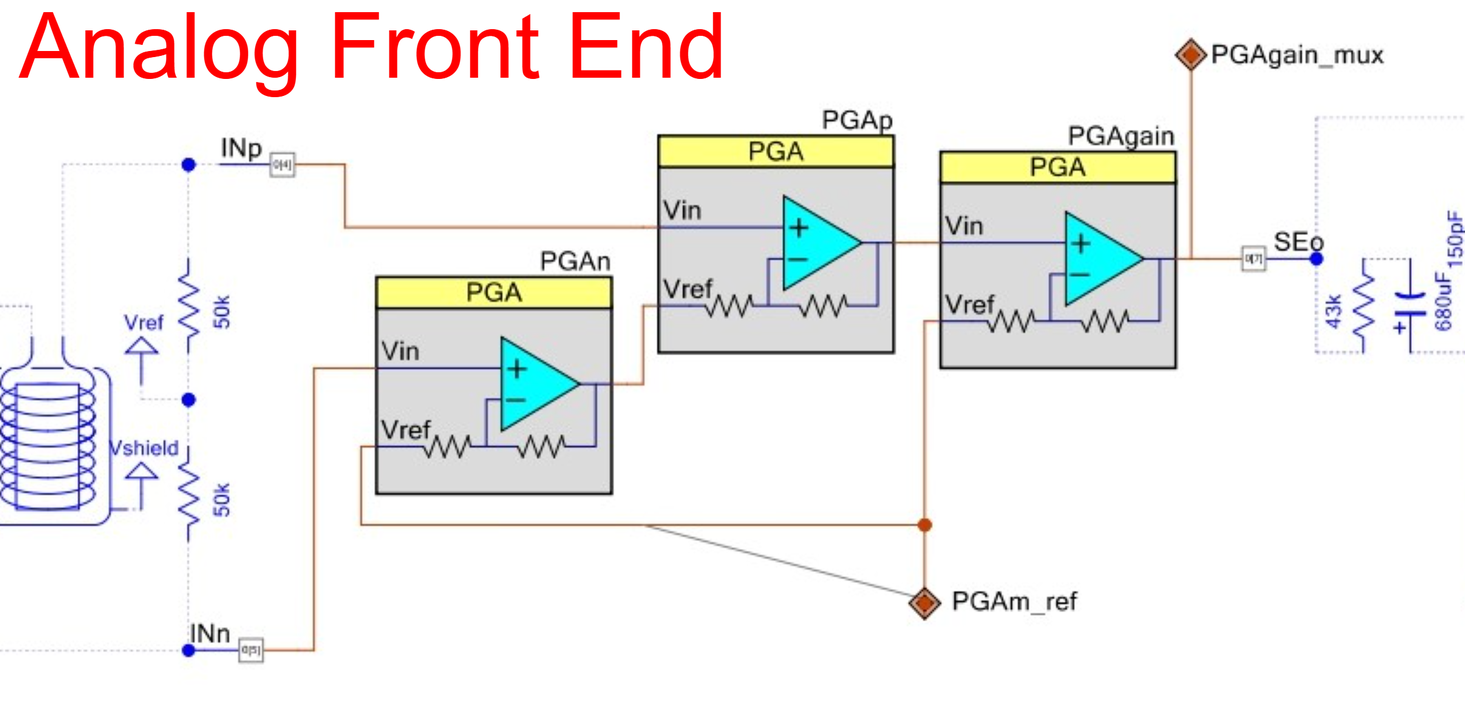
\includegraphics[width=\textwidth,keepaspectratio]{afe_entrada.png}\\[3mm]
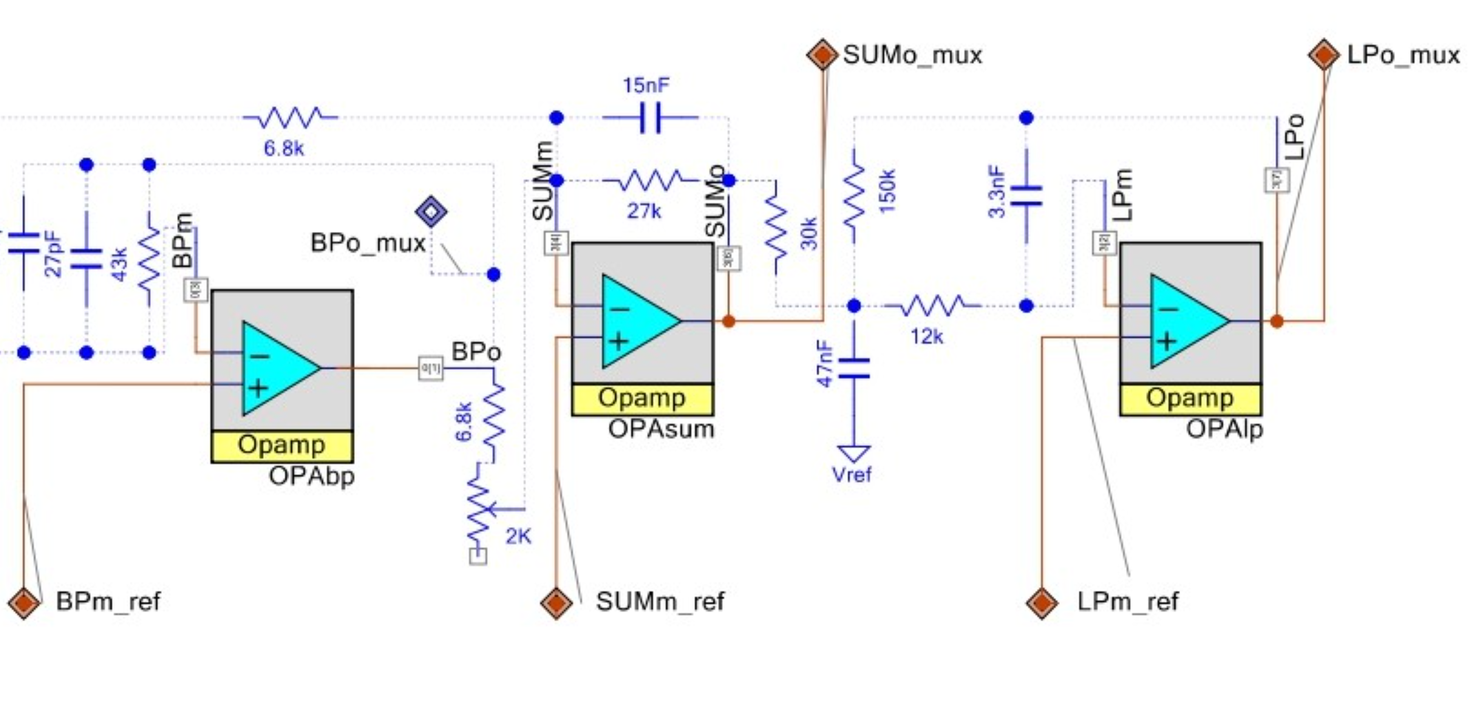
\includegraphics[width=\textwidth,keepaspectratio]{afe_compensa.png}
\caption{Cadena analógica implementada, en dos mitades del mismo esquemático.
Arriba: entrada
instrumental diferencial y etapa de ganancia programable.
Abajo: rama pasabanda de compensación en torno a \texttt{OPAbp}, con el
potenciómetro de 2\,k$\Omega$ que ajusta la cancelación, el sumador \texttt{OPAsum}
de 27\,k$\Omega$ y el pasa-bajos de realimentación múltiple \texttt{OPAlp}
(30\,k$\Omega$ / 150\,k$\Omega$ / 12\,k$\Omega$, 47\,nF y 3,3\,nF) previo al convertidor.}
\end{figure*}

El acondicionamiento implementado en el PSoC 5LP encadena una entrada instrumental, una etapa de ganancia programable, una rama de compensación, un sumador y un filtrado pasa-bajos previo a la conversión. La etapa de compensación es la decisión de diseño central del frente analógico y merece desarrollarse con detalle.

El punto de partida es que una misma tensión de salida del geófono admite dos lecturas. Referida a la velocidad del suelo, la respuesta del sensor es un pasa-altos de segundo orden,

\begin{equation}
H_v(s)=\frac{V_o(s)}{\dot X_g(s)}=-G_0\,\frac{s^{2}}{s^{2}+2\zeta_0\omega_n s+\omega_n^{2}},
\end{equation}

donde $G_0$ es la sensibilidad, $\omega_n=2\pi f_n$ la pulsación natural y $\zeta_0$ el amortiguamiento nominal. Como la aceleración cumple $A_g(s)=s\dot X_g(s)$, la misma salida referida a aceleración resulta

\begin{equation}
H_a(s)=\frac{H_v(s)}{s}=-G_0\,\frac{s}{s^{2}+2\zeta_0\omega_n s+\omega_n^{2}},
\end{equation}

que es un pasabanda y no presenta meseta con el amortiguamiento nominal. Por debajo de $f_n$, $|H_v|$ cae a razón de 40 dB por década y $|H_a|$ a 20 dB por década. No se trata de dos modos de funcionamiento sino de dos referencias de la misma tensión, y la distinción importa porque la estrategia de compensación se formula sobre la referencia a aceleración.

La observación que aporta Ma y colaboradores es que no hace falta invertir la respuesta del sensor, operación mal condicionada porque amplificaría el ruido con la misma pendiente con que el geófono atenúa la señal. Basta con conservar $f_n$ y elevar el amortiguamiento efectivo hasta un valor $\zeta_1\gg\zeta_0$, con lo cual la respuesta referida a aceleración se aplana entre

\begin{equation}
f_1\simeq\frac{f_n}{2\zeta_1},
\qquad
f_2\simeq 2\zeta_1 f_n,
\end{equation}

de modo que $\zeta_1$ se elige para llevar el quiebre inferior $f_1$ hasta la banda de interés. El quiebre superior $f_2$ no constituye un objetivo, ya que la aplicación no requiere extender la banda alta; sólo se conserva la simetría logarítmica $f_1f_2=f_n^{2}$ en torno a $f_n$.

La transferencia que realiza esa transformación es el cociente entre el denominador nominal y el deseado,

\begin{equation}
H_{\mathrm{comp}}(s)=\frac{s^{2}+2\zeta_0\omega_n s+\omega_n^{2}}{s^{2}+2\zeta_1\omega_n s+\omega_n^{2}},
\end{equation}

y al separar el término constante aparece la forma que da nombre a la arquitectura y que se implementa directamente en el circuito,

\begin{equation}
H_{\mathrm{comp}}(s)=1-\frac{2(\zeta_1-\zeta_0)\,\omega_n s}{s^{2}+2\zeta_1\omega_n s+\omega_n^{2}}.
\end{equation}

La estructura $1-\mathrm{BP}$ no es entonces una elección heurística sino una consecuencia algebraica: el camino directo menos un pasabanda centrado en la resonancia del sensor. Su implementación se resolvió desacoplando los dos polos, uno en la entrada y otro en la realimentación de un inversor, de manera que cada uno dependa de un único par $RC$. Esa realización se comparó experimentalmente contra una Sallen-Key y contra una de realimentación múltiple. La Sallen-Key quedó descartada porque su realimentación positiva agrava la sensibilidad del $Q$ a las tolerancias y admite oscilación si los componentes se apartan del valor nominal, mientras que la desviación medida respecto de la respuesta objetivo resultó menor en la realimentación múltiple. Conviene precisar que esta última no se abandonó: es la topología con la que está implementado el filtro pasa-bajos antialias que precede al convertidor. Los valores se resolvieron por búsqueda sobre la malla de componentes comerciales incorporando el modelo no ideal del amplificador del PSoC, y un potenciómetro en serie con la rama pasabanda permite ajustar en cada unidad la proporción de la que depende la cancelación.

\begin{figure*}[!tb]
\centering

\includegraphics[width=\textwidth,keepaspectratio]{extension_banda.png}
\caption{Efecto de la compensación sobre la respuesta referida a aceleración. Al elevar $\zeta_1$ los polos complejos se separan en dos reales, y el inferior desplaza el quiebre $f_1$ hacia la banda de interés.}
\end{figure*}

El precio de la compensación es alto y conviene explicitarlo, porque condiciona todo el resto del frente analógico. Con los valores implementados se obtiene $f_0=10{,}20$ Hz y un amortiguamiento efectivo $\zeta_1\simeq 937$, que es el valor con el que se diseñó la rama pasabanda. En la zona central la respuesta compensada queda escalada por $1/(2\zeta_1)\simeq 5{,}3\times10^{-4}$, esto es, una atenuación cercana a 1875 veces que debe recuperarse íntegramente en ganancia. Esa ganancia se repartió deliberadamente entre etapas para no concentrar el margen en un solo bloque: la entrada instrumental aporta $\times 2$, la etapa programable entre $\times 1$ y $\times 50$, el sumador $\times 3{,}6$ sobre la rama de compensación y el pasa-bajos $\times 5$, con un producto máximo de $\times 1800$. El propósito de la compensación no es convertir al SM-24 en un sensor de banda ancha, objetivo inalcanzable por vía puramente electrónica, sino conservar una forma de respuesta predecible en la banda baja y aprovechar el margen del convertidor, aceptando a cambio un compromiso explícito con el ruido: toda la cadena de ganancia que restituye ese factor 1875 amplifica también el ruido propio del frente, y es esa tensión la que vuelve indispensables las mediciones de ruido referido a entrada que la sección 12 declara pendientes.

Extender la banda hacia baja frecuencia agrava el problema del offset y de la deriva, que de otro modo consumirían el rango del convertidor sin aportar señal. Para controlarlo, un multiplexor permite observar nodos internos de la cadena con el mismo convertidor, y una rutina de calibración en primer plano ajusta secuencialmente las referencias de la etapa de ganancia, de la rama de compensación, del sumador y del filtro. Durante la captura los lazos se desactivan y se aplican códigos fijos almacenados con verificación de integridad, de manera que ninguna corrección actúe sobre la señal mientras se registra. La revisión posterior del circuito, que sustituye las referencias por fuentes de corriente e incorpora una etapa de ganancia de salida, se encuentra en desarrollo y no participó de la campaña; los resultados de la sección 10 corresponden exclusivamente a la ruta anterior.

\begin{figure*}[!tb]
\centering
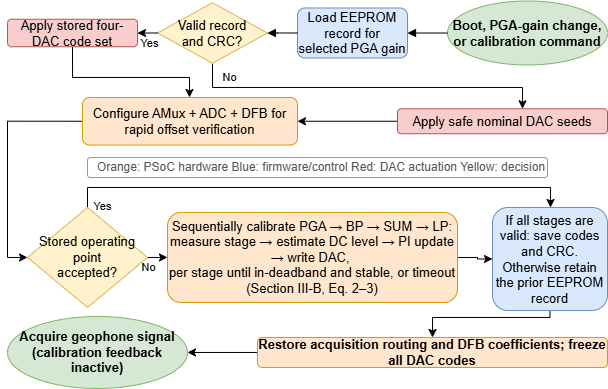
\includegraphics[width=0.62\textwidth,keepaspectratio]{flujo_calibracion_horizontal_usuario.png}
\caption{Flujo de la calibración \emph{foreground}: las etapas se ajustan en orden, cada una hasta entrar en su banda muerta, y la adquisición se restaura con códigos fijos.}
\end{figure*}

\subsection{Digitalización y temporización determinista}

\begin{figure*}[!tb]
\centering
\begin{minipage}[t]{0.53\textwidth}\centering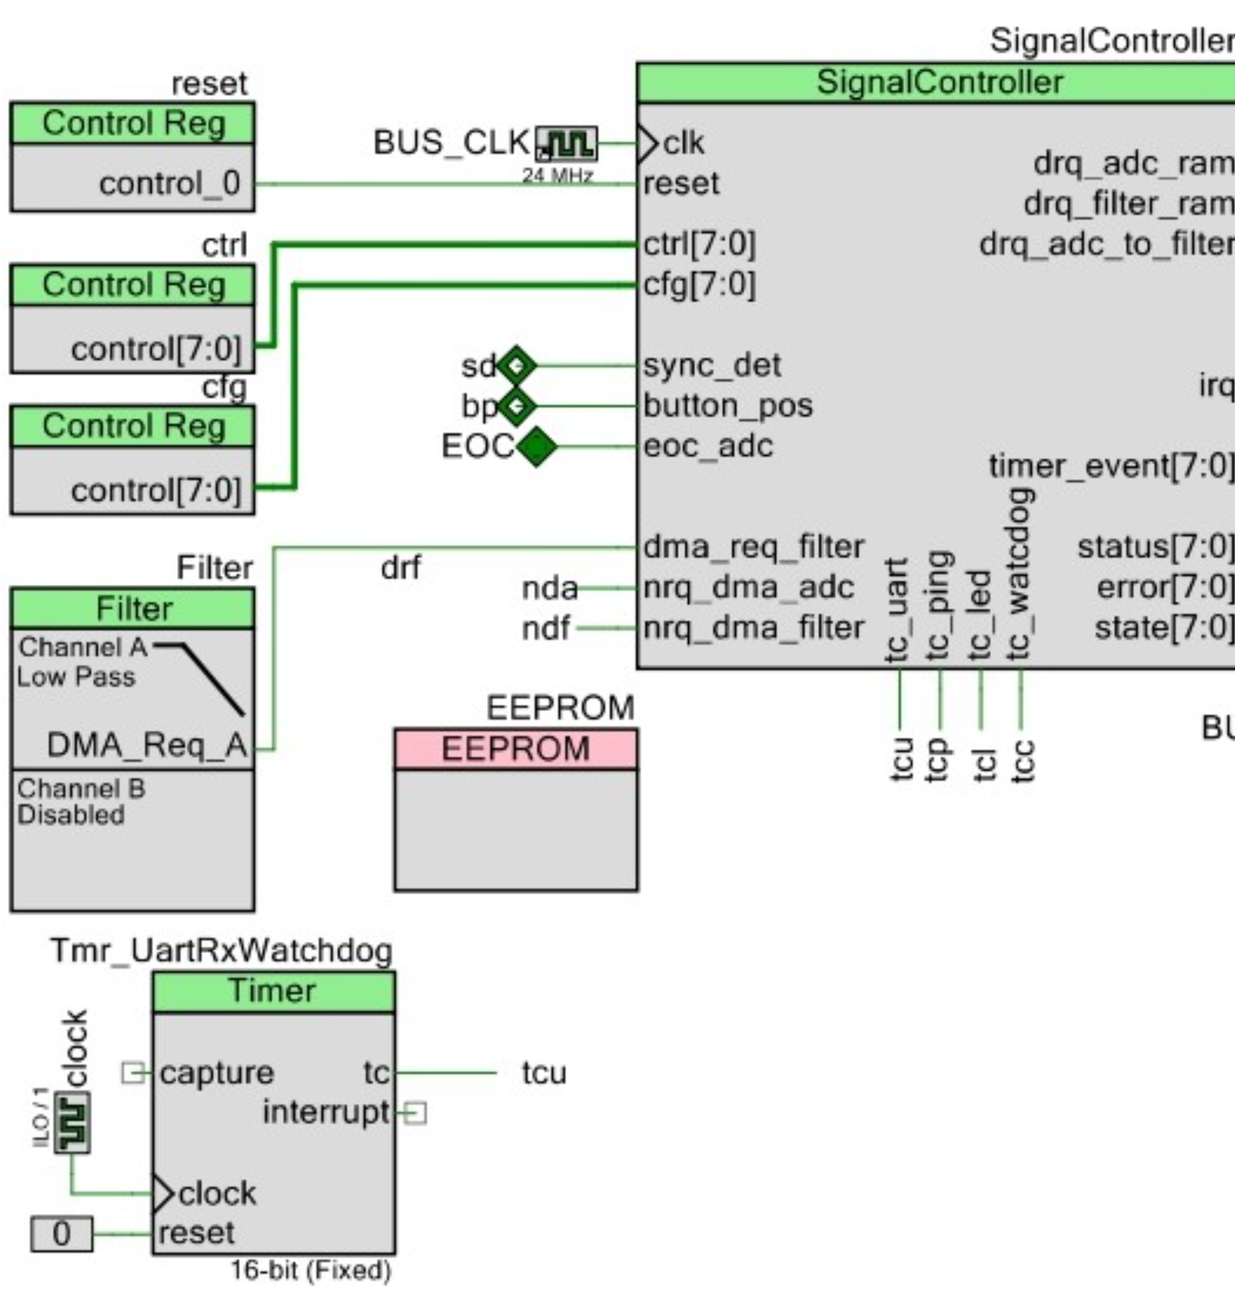
\includegraphics[width=\textwidth,keepaspectratio]{dig_control.png}\end{minipage}\hfill
\begin{minipage}[t]{0.44\textwidth}\centering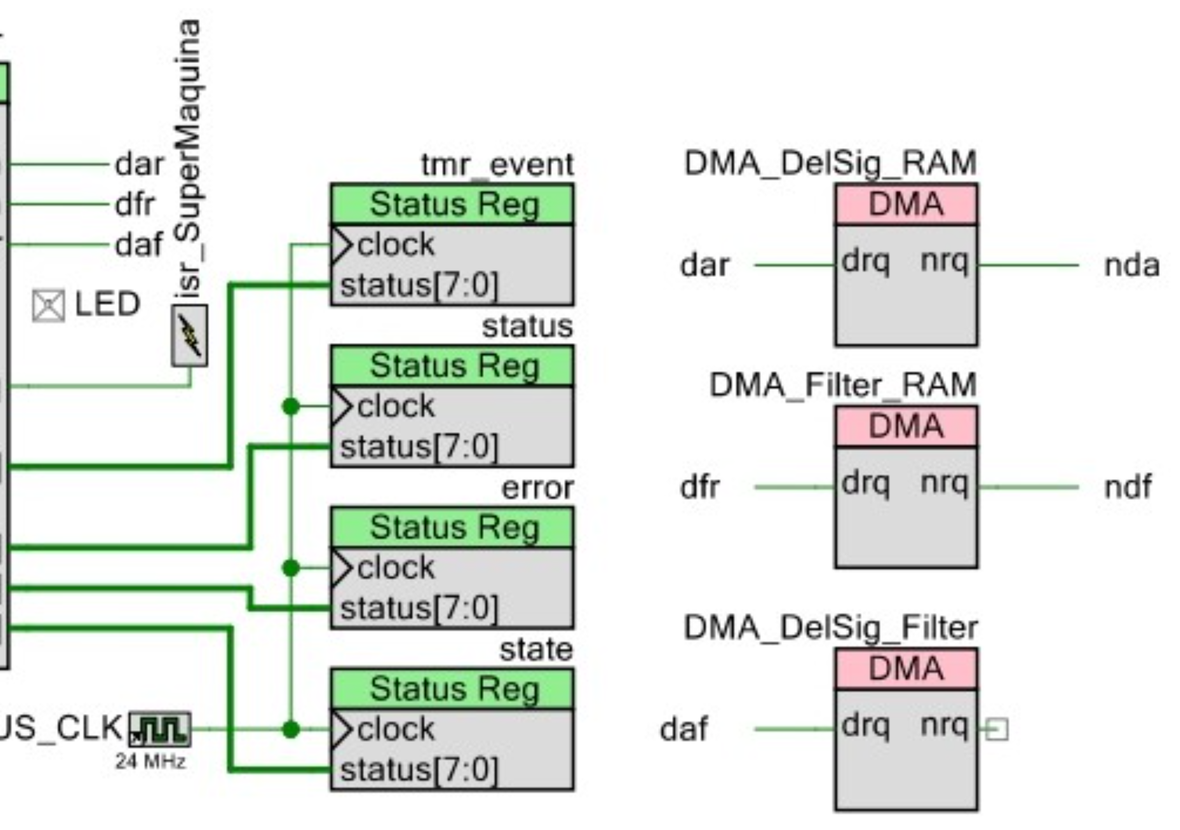
\includegraphics[width=\textwidth,keepaspectratio]{dig_dma.png}\end{minipage}
\caption{Camino digital implementado en el PSoC. Izquierda: bloque de control
\texttt{SignalController} descrito en lógica programable, con los registros de
configuración, el filtro FIR por hardware y el temporizador de vigilancia.
Derecha: registros de estado y los tres canales de acceso directo a memoria que
trasladan la señal cruda y la filtrada sin intervención del procesador.}
\end{figure*}

La conversión emplea el convertidor delta-sigma del PSoC configurado a una frecuencia de muestreo del orden de 2604 muestras por segundo, con resolución nominal de 18 bits y rangos bipolares seleccionables que se coordinan con la ganancia programable para aprovechar la escala sin saturar. Un filtro FIR implementado en hardware y varios canales de acceso directo a memoria trasladan la señal cruda y la filtrada sin intervención del procesador.

La elección de una arquitectura delta-sigma frente a una de aproximaciones sucesivas responde a la forma particular del problema. La banda de interés termina por debajo de unos pocos cientos de hertz, de modo que la velocidad de conversión no es una restricción, mientras que el rango dinámico sí lo es: el mismo registro debe contener el primer arribo cercano a la fuente y la llegada atenuada del offset más lejano. Un convertidor delta-sigma explota precisamente ese desbalance, ya que sobremuestrea muy por encima de la banda útil y desplaza el ruido de cuantificación hacia frecuencias altas, donde el diezmado lo elimina; obtiene así una resolución que una arquitectura de aproximaciones sucesivas sólo alcanzaría con un comparador y una referencia considerablemente más costosos. El sobremuestreo aporta una segunda ventaja relevante en campo: relaja la exigencia sobre el filtro antialias analógico, cuyo orden y precisión de componentes habrían tenido que aumentar para proteger una conversión directa a esa velocidad. A ello se suma que el convertidor está integrado en el mismo dispositivo que aloja el acondicionamiento y la lógica de control, lo que evita una interfaz externa y sus problemas asociados de acoplamiento y de temporización.

La temporización de la ventana de captura es el punto donde la sección 8 impone su condición más estricta, y por eso no se delegó al software. Una máquina de estados descrita en lógica programable coordina el disparo, la habilitación del convertidor, el conteo de muestras y el cierre de la captura, de modo que la duración y el instante de la ventana no dependen de la latencia variable del firmware. Esta decisión es la que hace defendible el requerimiento de sincronización, aunque su verificación experimental siga pendiente. Queda además una decisión de diseño abierta que incide directamente sobre esa métrica: la selección de la fuente de reloj que gobierna la ventana. El oscilador interno del dispositivo resulta suficiente para fijar la duración de la captura, pero su deriva y su incertidumbre de frecuencia se acumulan sobre registros largos y entre nodos distintos, de modo que evaluar un cristal externo o una referencia compartida es parte del trabajo necesario para acercarse a la tolerancia derivada en la sección 8.

Corresponde una advertencia explícita sobre la resolución. Los 18 bits son una cifra nominal del convertidor y no un número efectivo de bits medido: faltan ensayos de ruido referido a entrada, linealidad, saturación y repetibilidad por rango y por ganancia. Que la campaña haya registrado señales utilizables demuestra que la cadena funciona, no que su desempeño esté cuantificado.

\subsection{Sincronización, comunicaciones y trazabilidad}

La coordinación entre nodos y el transporte de datos se resuelven sobre módulos ESP32 mediante un protocolo de difusión directa entre pares, que evita depender de infraestructura de red en campo. Como una captura completa excede ampliamente la carga útil de un paquete y el enlace no garantiza entrega, el protocolo fragmenta cada registro, numera las secuencias, confirma la recepción y reintenta los fragmentos faltantes, mientras cada nodo conserva además una copia local. El motivo de exigir la entrega íntegra, y no una reconstrucción aproximada, es que la magnitud que el método estima es una fase: un tramo de muestras faltante no degrada gradualmente el resultado sino que invalida el registro completo para el cálculo de dispersión. De ahí que la política ante una pérdida sea reintentar o descartar, y que la copia local exista precisamente para que descartar no signifique perder la posición.

La separación entre la interfaz de campo, que opera los nodos, y el servidor, que valida, agrupa y preserva los registros junto con su geometría y sus metadatos, es la que permite reconstruir a posteriori cualquier resultado a partir de los datos almacenados.

\subsection{Fuente instrumentada}

La excitación se aplica con un martillo instrumentado PCB 086D20, cuyo sensor piezoeléctrico de tipo ICP entrega una medida de la fuerza aplicada y requiere alimentación por corriente constante con desacople de la polarización \citep{PCB086D20,PCBSignalConditioning}; el acondicionamiento correspondiente se integró en el mismo PSoC. El nodo HAMMER y el nodo GEO se adquieren de forma conjunta y con arranque coordinado, lo que permite referenciar cada respuesta al instante del impacto y, sobre todo, apilar varios golpes por posición.

La repetibilidad de la fuente adquiere una importancia particular en el protocolo empleado. Cuando el arreglo se construye desplazando un receptor, cualquier variación de amplitud, punto de golpe o acoplamiento entre posiciones sucesivas se incorpora al registro como si fuera variación espacial. Registrar entre veinte y treinta y siete golpes por posición y seleccionar el subconjunto más consistente reduce ese riesgo pero no lo elimina, y por esa razón la geometría aparece en la sección 11 como la sensibilidad dominante del resultado.


\begin{figure*}[!tb]
\centering

\includegraphics[width=\textwidth,keepaspectratio]{repetibilidad_fuente.png}
\caption{Repetibilidad del impacto medida sobre el canal del martillo. Los puntos claros son golpes individuales y las líneas la mediana por posición.}
\end{figure*}
\section{Validación experimental}
\label{sec:validacion}

La validación se organiza en los tres niveles que corresponden a un trabajo de instrumentación: la caracterización electrónica del instrumento, una prueba controlada de adquisición y una campaña de campo representativa. El caso de campo se presenta como demostración de la utilidad del instrumento y no como un estudio geofísico autónomo.

\subsection{Caracterización electrónica del frente analógico}
\label{sec:ensayo-electronico}

El ensayo buscó evaluar si la respuesta del compensador, combinada con la del geófono, permite extender el ancho de banda del sensor hacia frecuencias inferiores a su resonancia. Se inyectaron barridos senoidales de tensión y se registraron simultáneamente, con cuatro canales de osciloscopio, las salidas de la ganancia programable, la rama pasabanda, el compensador y el filtro pasa-bajos. A partir de las relaciones entre canales se estimaron la magnitud, la fase y la coherencia de cada transferencia. Los barridos cubrieron bandas superpuestas desde 10 mHz hasta 200 kHz.

El estimador empleado opera con las señales analíticas de entrada $u_a[n]$ y salida $y_a[n]$, obtenidas mediante la transformada de Hilbert. Para las muestras $\mathcal B_k$ del intervalo de frecuencia $k$:
\begin{equation}
\begin{aligned}
C_k&=\sum_{n\in\mathcal B_k}y_a[n]u_a^*[n],\\
E_{u,k}&=\sum_{n\in\mathcal B_k}|u_a[n]|^2,\qquad
E_{y,k}=\sum_{n\in\mathcal B_k}|y_a[n]|^2,\\
\widehat H_k&=\frac{C_k}{E_{u,k}},\qquad
\gamma_k^2=\frac{|C_k|^2}{E_{u,k}E_{y,k}}.
\end{aligned}
\label{eq:estimacion-transferencia}
\end{equation}
El asterisco indica conjugación compleja, $\widehat H_k$ es la transferencia estimada y $\gamma_k^2$ la coherencia. Se excluyen intervalos saturados o con excitación insuficiente.

La respuesta conjunta sensor--acondicionamiento se calculó combinando el modelo nominal del geófono con la transferencia electrónica medida. Un ensayo con el sensor sometido a una excitación mecánica conocida permitiría verificar directamente esa respuesta, pero no se dispuso del equipo necesario. La inyección de tensión permitió caracterizar por separado el circuito y evaluar su contribución a la extensión de banda.

Para comparar las mediciones con el diseño se consideraron dos intervalos: el generado por las tolerancias de los componentes, manteniendo el potenciómetro en el ajuste nominal, y el alcanzable al recorrer el potenciómetro. La tabla~\ref{tab:envolventes} presenta la proporción de puntos comprendidos en cada intervalo.

\begin{table*}[!ht]
\centering
\footnotesize
\caption{Identificación de las etapas y ubicación de la medición respecto de
dos envolventes: la de tolerancias de componente con el potenciómetro en su valor de
diseño, y la que barre todo el recorrido del potenciómetro. \revsolution{Fuente: elaboración propia.}}
\label{tab:envolventes}
\begin{tabularx}{0.92\textwidth}{YYYYYY}
\toprule
Ruta medida & Puntos & Banda identificada & Coherencia & Dentro de tolerancias (mag./fase) & Dentro del recorrido del pot.\ (mag./fase) \\
\midrule
BP & 85 & 0,21 Hz – 47,5 kHz & 0,9684 & 32 \% / 6 \% & 32 \% / 6 \% \\
Compensador & 71 & 0,21 Hz – 4,74 kHz & 0,9643 & 37 \% / 11 \% & \textbf{92 \% / 94 \%} \\
LP & 33 & 11,75 Hz – 1,11 kHz & 0,9454 & 82 \% / 94 \% & 82 \% / 94 \% \\
\textbf{PGA → ADC (ruta completa)} & \textbf{61} & \textbf{0,21 Hz – 1,11 kHz} & \textbf{0,9946} & 41 \% / 15 \% & \textbf{100 \% / 100 \%} \\
\bottomrule
\end{tabularx}
\end{table*}

En la ruta completa PGA--ADC, el 100 \% de los puntos queda dentro del intervalo alcanzable con el potenciómetro, tanto en magnitud como en fase; para el compensador, las proporciones son del 92 \% y del 94 \%. La respuesta de la cadena es, por tanto, compatible con el rango de ajuste previsto. Las tolerancias por sí solas, con el potenciómetro fijo en su valor nominal, no explican toda la diferencia: la posición del ajuste es determinante.

\begin{figure*}[!tb]
\centering
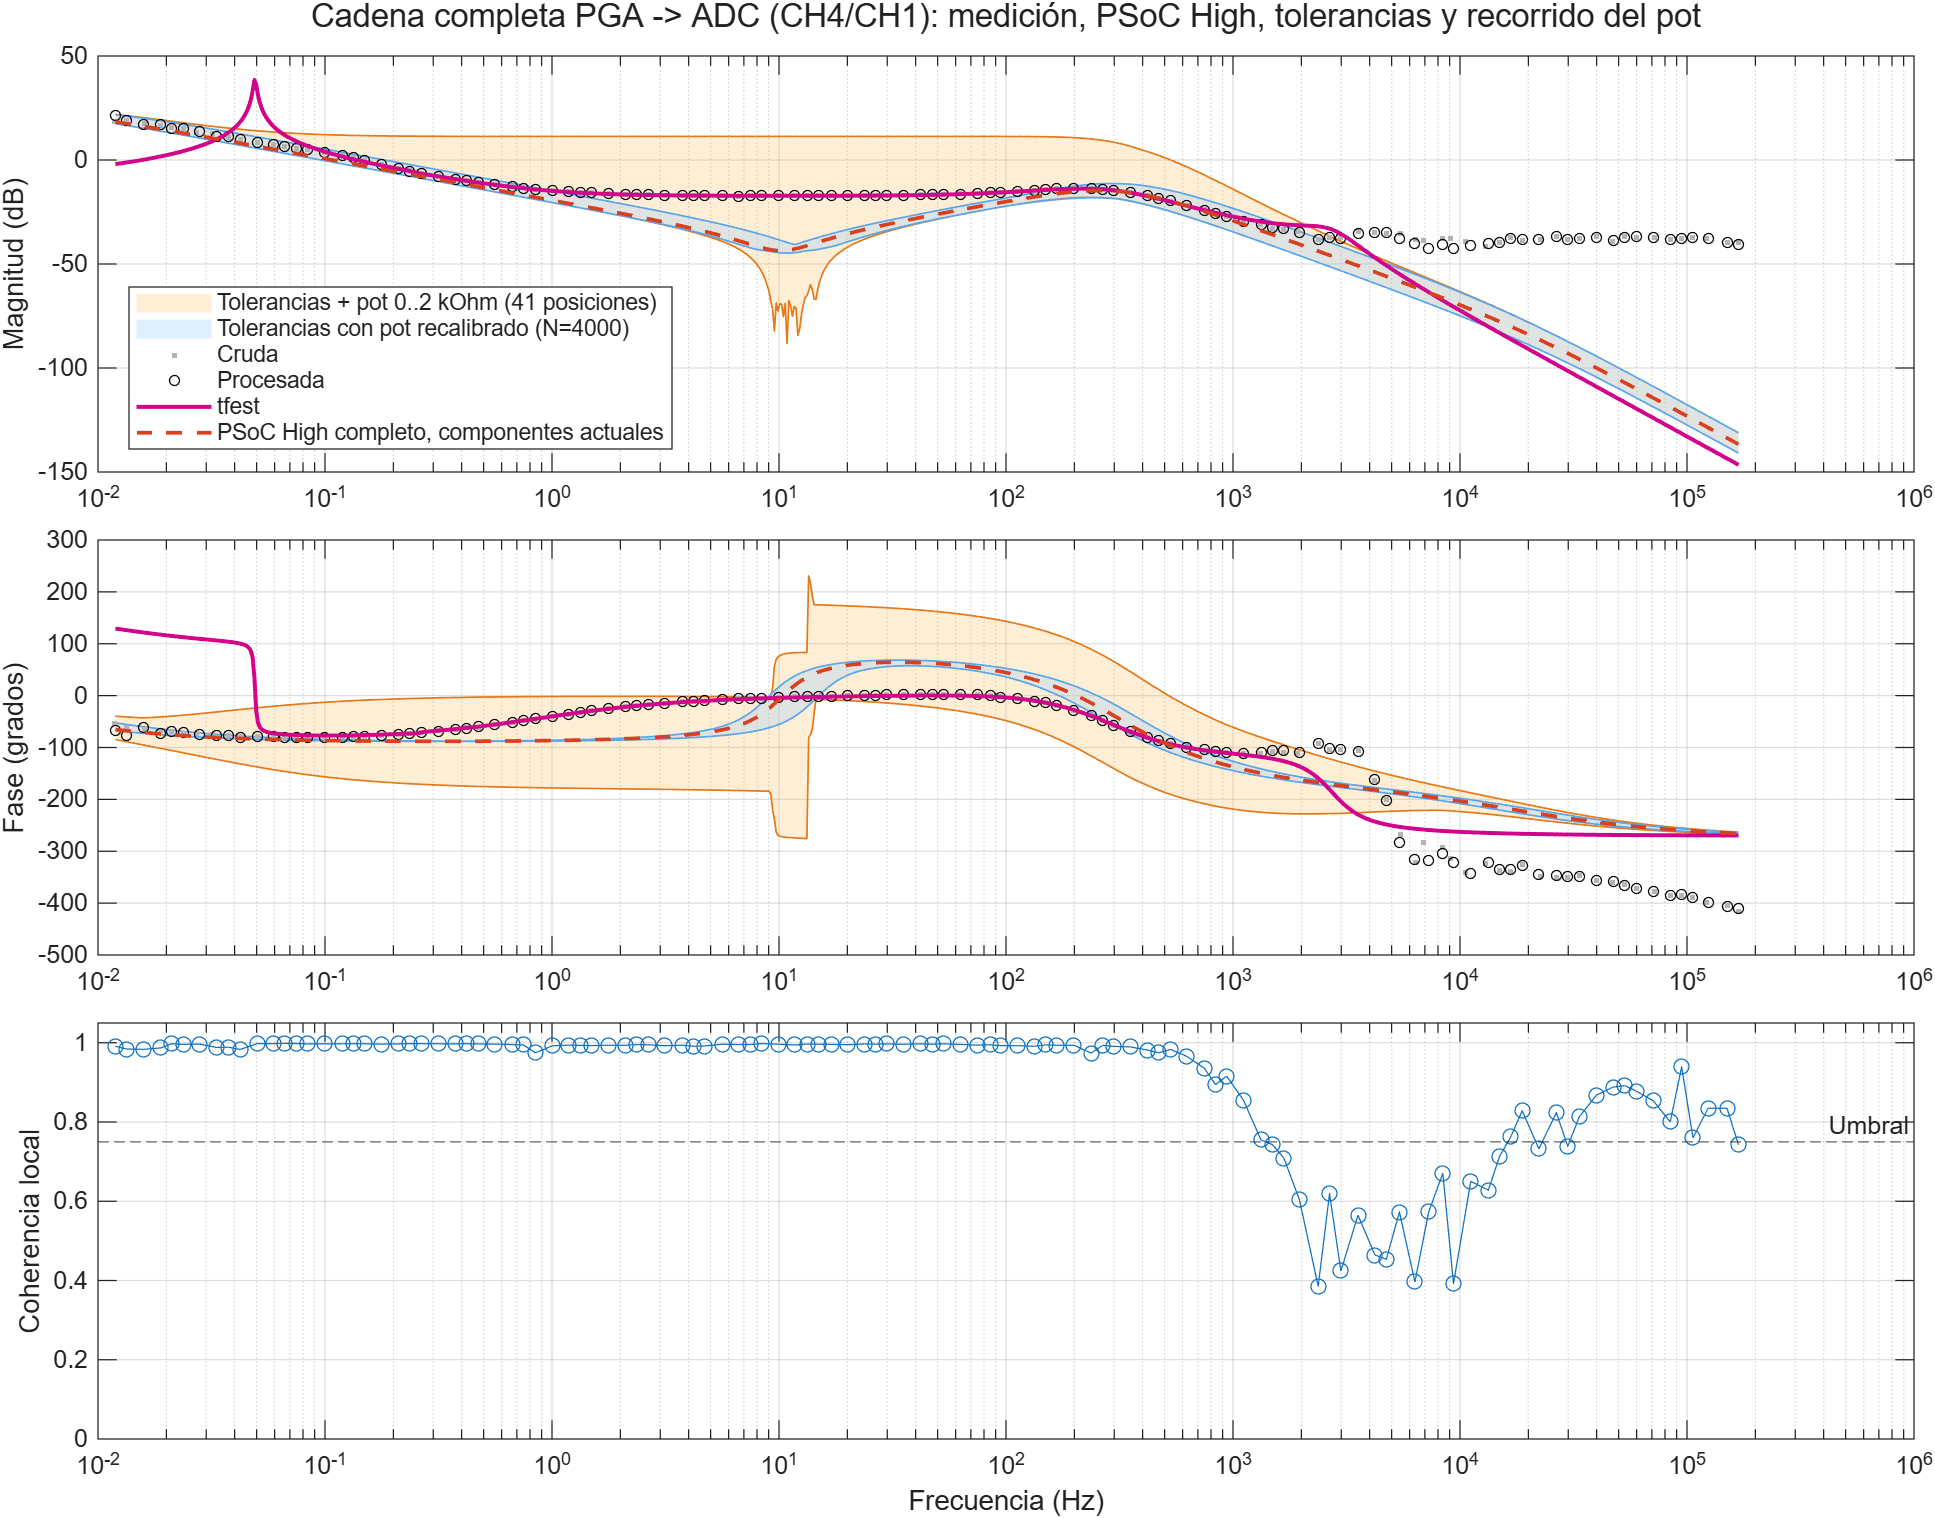
\includegraphics[width=\textwidth,keepaspectratio]{f_ruta_pga_adc.png}
\caption{Identificación de la cadena completa PGA--ADC. De arriba abajo: magnitud, fase y coherencia local. Se comparan la medición cruda, la procesada, el modelo identificado y el modelo nominal del circuito con los componentes actuales. \revsolution{Fuente: elaboración propia a partir de los registros del proyecto.}}
\label{fig:identificacion}
\end{figure*}

\begin{figure*}[!tb]
\centering
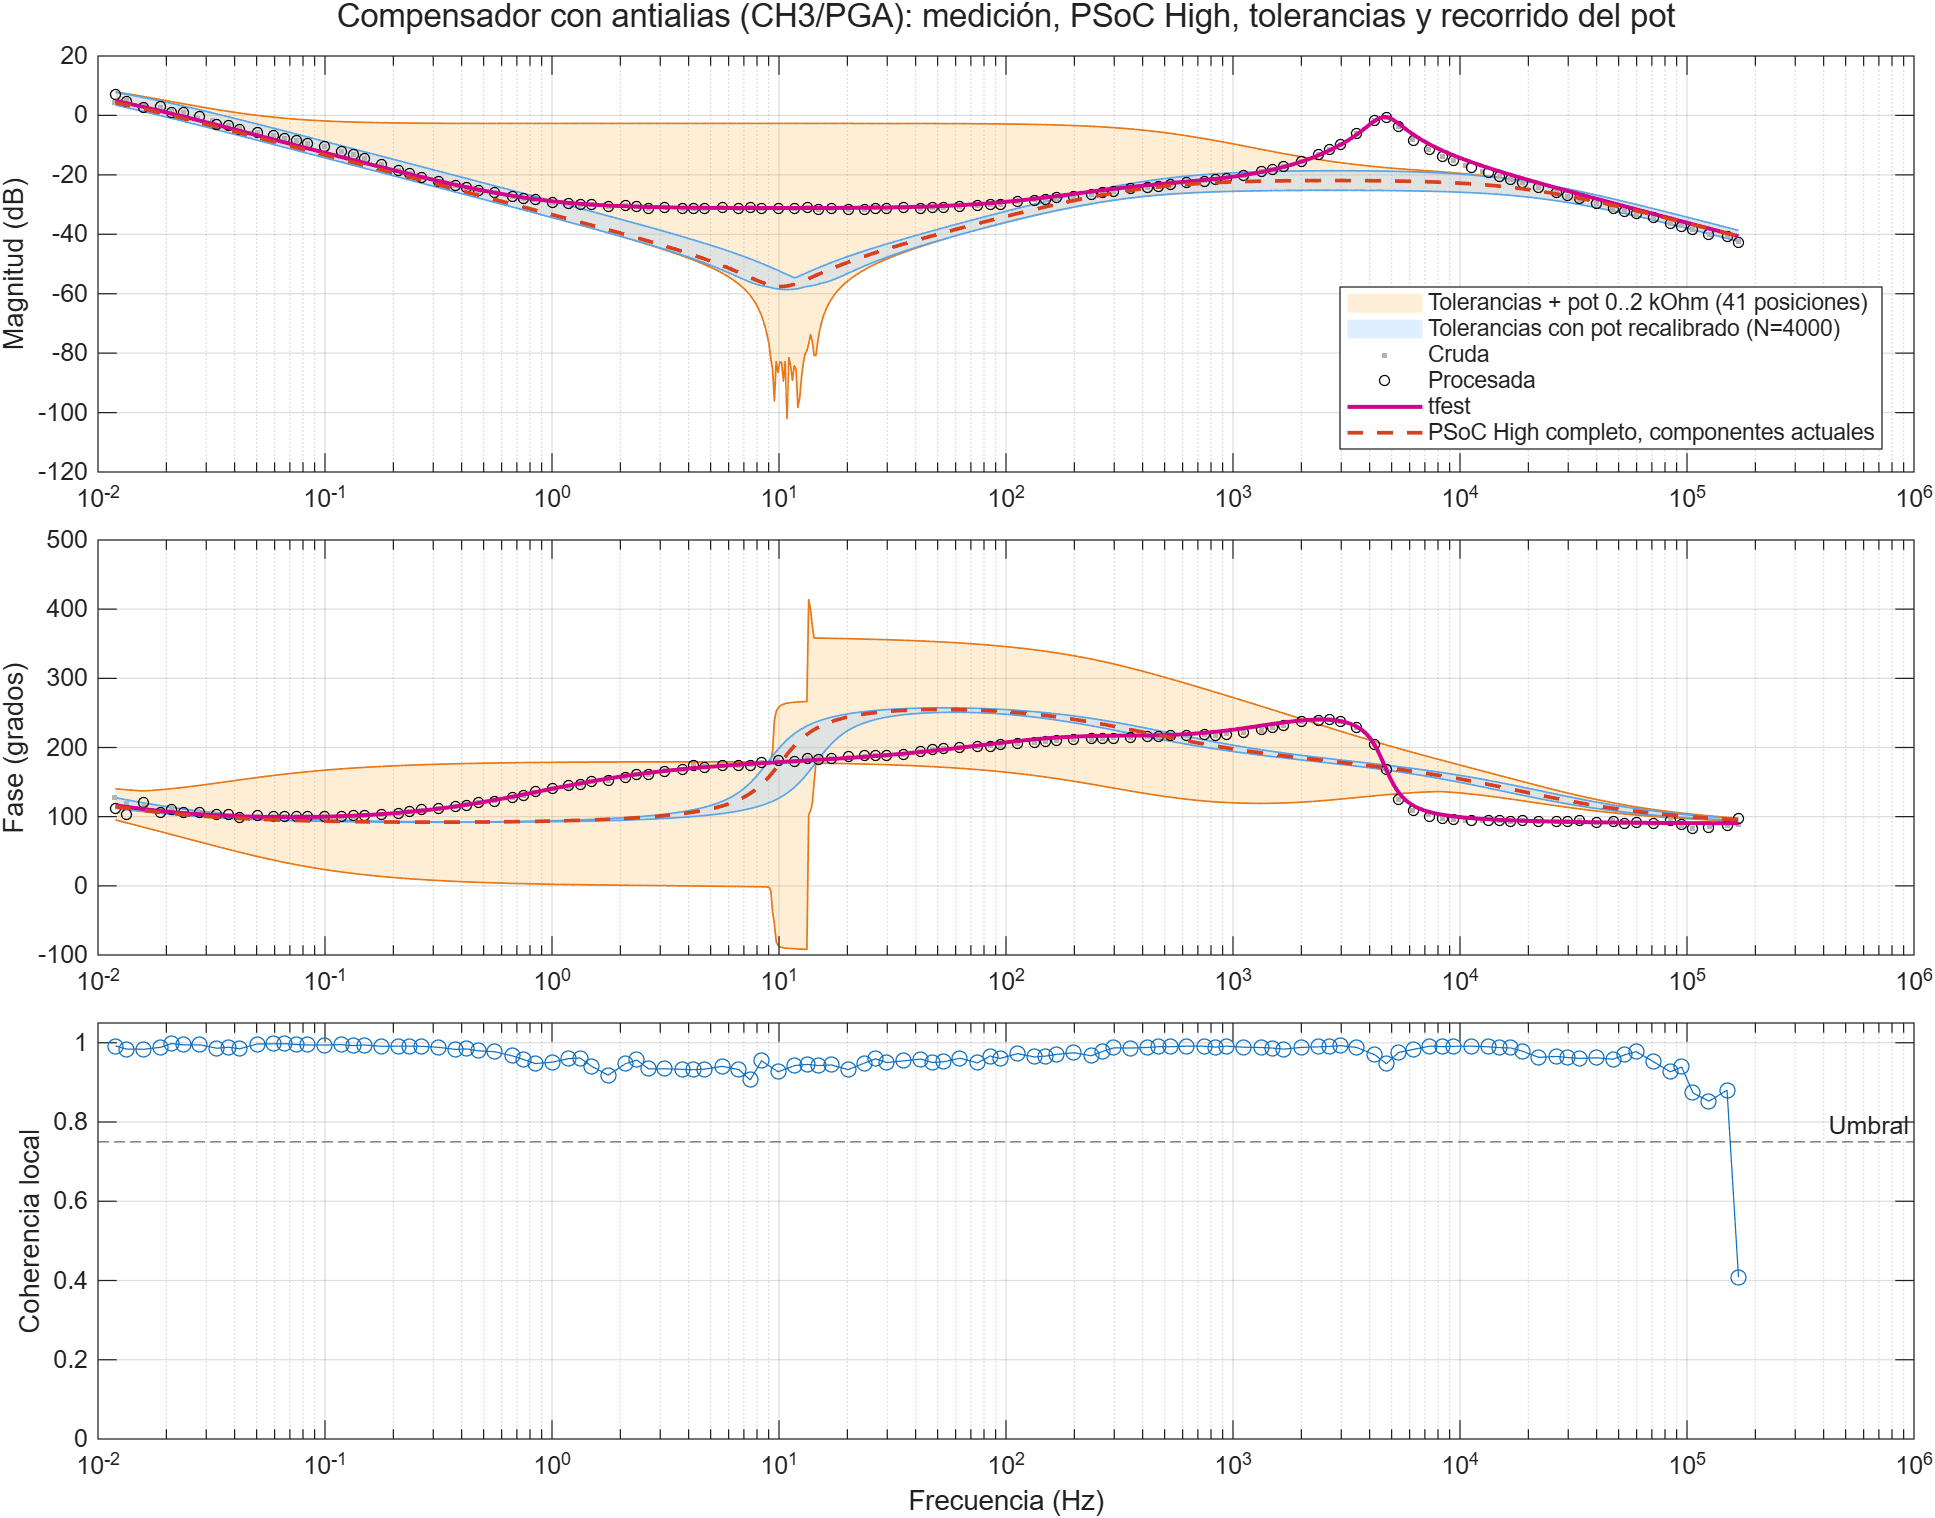
\includegraphics[width=\textwidth,keepaspectratio]{f_identificacion_comp.png}
\caption{Identificación de la rama de compensación respecto de la etapa de ganancia. El apartamiento respecto del modelo nominal se explica por la posición del potenciómetro y no por un componente fuera de especificación. \revsolution{Fuente: elaboración propia a partir de los registros del proyecto.}}
\label{fig:identificacioncomp}
\end{figure*}

El aprendizaje principal fue la sensibilidad de la cancelación al valor del potenciómetro. Con los componentes nominales, la cancelación exacta y el ajuste objetivo están separados por apenas 1,98 $\Omega$ sobre un recorrido de 2 k$\Omega$. La calibración manual redujo el error de magnitud del compensador respecto del modelo de 26,7 a 10,7 dB, pero el ajuste fino resulta difícil con el elemento actual. Se propone mantener la resistencia fija de la rama y utilizar un potenciómetro de menor recorrido y varias vueltas, dimensionado para cubrir la dispersión esperada de los componentes.

La precisión de ese ajuste adquiere mayor importancia en un arreglo de varios receptores. Diferencias entre componentes o entre posiciones de los potenciómetros modifican la magnitud y la fase de cada canal; la diferencia de fase entre circuitos se incorpora entonces a la que el método utiliza para estimar la propagación. El ajuste multivuelta facilitará igualar las respuestas, que deberán comprobarse experimentalmente entre placas.

La ruta PGA--ADC quedó identificada sobre 61 puntos, entre 0,21 Hz y 1,11 kHz, con coherencia mediana de 0,9946. El modelo identificado reproduce esos datos con residuos de 0,200 dB y 1,16°; estos valores describen el ajuste a la medición, no el error respecto de la respuesta nominal.

\subsection{Prueba controlada de adquisición}
\label{sec:prueba-controlada}

El segundo nivel verifica que el sistema adquiere de forma coordinada antes de exigirle un resultado geofísico. El nodo generador se trata como un esclavo más y comparte el arranque con el nodo receptor, de modo que cada respuesta queda referida al instante de su impacto. Para cuantificar esa referencia se midió, dentro de cada posición, la dispersión entre los instantes de disparo de los golpes individuales una vez alineados a nivel de submuestra, obteniéndose un valor del orden de 1,46 ms. Conviene precisar qué describe y qué no describe ese número. Es el residuo de repetibilidad entre golpes sucesivos de un mismo nodo, y agrupa el jitter mecánico del impacto con el del circuito de disparo. No mide, en cambio, ni la deriva entre jornadas de adquisición ni la incertidumbre de la posición del receptor, que son fuentes de error independientes y se tratan como parte del problema de geometría y repetibilidad de la campaña en las secciones~\ref{sec:campana} y~\ref{sec:limitaciones}.

Para $M$ golpes alineados, la traza promedio $\bar x[n]$ se obtiene de los registros $x_m[n]$ y sus desplazamientos estimados $\delta_m$:
\begin{equation}
\bar x[n]=\frac{1}{M}\sum_{m=1}^{M}x_m[n+\delta_m].
\label{eq:apilamiento}
\end{equation}
Los desplazamientos pueden ser fraccionarios y requerir interpolación. Si la señal se repite y el ruido es independiente entre golpes, su desviación estándar se reduce idealmente como $\sigma_{\bar n}=\sigma_n/\sqrt M$ \revsolution{\citep{Smith1997}}. Se registraron entre 20 y 37 golpes por posición; el apilamiento no elimina las variaciones de posición o de acoplamiento entre registros.

La capa de coordinación entre nodos sí fue probada de forma independiente. En laboratorio se operaron tres nodos simultáneos, uno de clase HAMMER y dos de clase GEO, que ejecutaron correctamente el arranque conjunto y el reparto de la orden de captura. Este ensayo se realizó sobre los módulos de radio sin el acondicionamiento analógico ni el PSoC asociados, de modo que demuestra que el protocolo de coordinación escala más allá de dos nodos y opera como fue diseñado, pero no aporta una cifra de precisión: no hubo conversión sincrónica de señal ni registros exportados que permitan comparar marcas temporales.

Conviene por eso separar cuatro magnitudes que resulta fácil confundir. La primera es la alineación de golpes recién mencionada, que corresponde al procesamiento de un solo nodo. La segunda es la operación funcional de la coordinación multinodo, demostrada con los tres nodos de laboratorio. La tercera es la sincronización digital medida entre nodos distintos, que exige registros simultáneos y una comparación de marcas temporales entre placas completas, y que no pudo realizarse por no disponerse de un conjunto de nodos GEO íntegros. La cuarta es la verificación instrumental del arranque coordinado mediante osciloscopio, que llegó a observarse durante el desarrollo pero cuyos registros no fueron preservados y que por lo tanto no constituye evidencia reproducible. La tolerancia de unos 670 µs derivada en la sección~\ref{sec:requerimientos} permanece, en consecuencia, como requerimiento de diseño cuya capa funcional está demostrada y cuya verificación metrológica está pendiente.

\subsection{Campaña de campo}
\label{sec:campana}

La campaña se realizó junto a una cancha de fútbol del predio de la Universidad Católica, sede Santa Librada, en Asunción. El punto de impacto permaneció fijo a varios metros del extremo del campo de fútbol y solamente se desplazó el nodo receptor, siguiendo una línea aproximadamente paralela a los laterales de la cancha. No se conservaron coordenadas ni azimut de los extremos del tendido, limitación que se retoma en la sección~\ref{sec:limitaciones}.

Se relevaron 21 posiciones entre 10 y 50 m de offset, con paso nominal de 2 m y una apertura total de 40 m, valores que corresponden a los límites de aliasing y de apertura establecidos en la sección~\ref{sec:requerimientos}. Del conjunto de 607 registros candidatos, 598 fueron incorporados al conjunto procesado tras la auditoría de calidad, con una mediana cercana a 30 golpes por posición. El arreglo se construyó desplazando un único receptor entre posiciones debido al número de transductores disponibles.

\begin{figure*}[!tb]
\centering
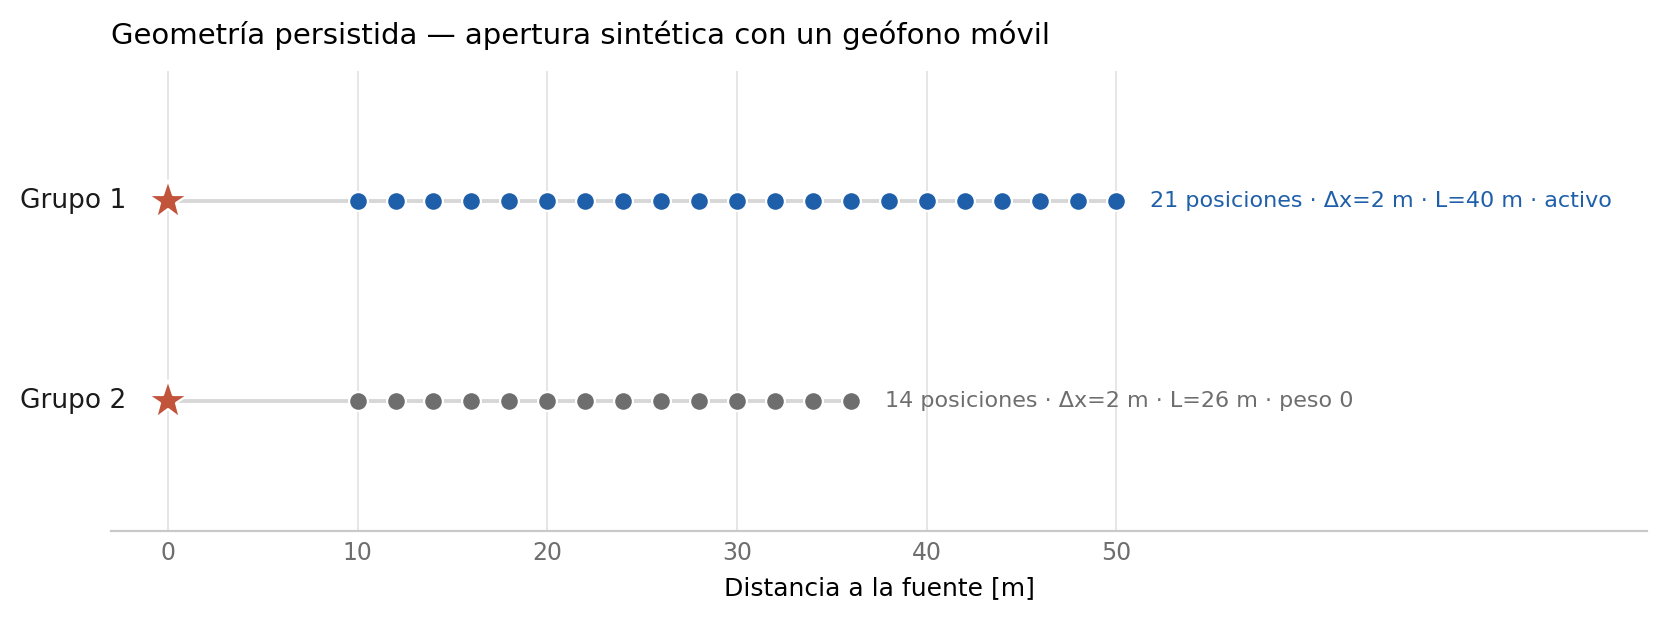
\includegraphics[width=\textwidth,keepaspectratio]{f_geometria_campanas.png}
\caption{Geometría de la campaña: 21 posiciones entre 10 y 50 m de offset con paso nominal de 2 m, lo que da una apertura total de 40 m. El arreglo se construyó desplazando un único receptor entre posiciones sucesivas. \revsolution{Fuente: elaboración propia a partir de los registros del proyecto.}}
\label{fig:geometria}
\end{figure*}

Esa restricción define con precisión qué valida la campaña. El conjunto permite construir un \textbf{registro multicanal sintetizado por posiciones con fuente activa repetible}, y sobre él evaluar la adquisición real, formar una imagen de dispersión e invertir un perfil preliminar. No demuestra, en cambio, la operación de 21 canales físicos simultáneos, ni la sincronización entre nodos, ni la igualdad de magnitud y fase entre placas distintas. La expresión «adquisición simultánea de 21 canales» sería incorrecta y no se emplea en ningún punto de este trabajo. Conviene señalar que el uso de un solo receptor no carece de antecedentes formales: Lin y Ashlock demostraron que la simulación multicanal con un receptor puede producir imágenes de dispersión comparables a las de MASW bajo condiciones controladas, si bien su protocolo fija el receptor y desplaza la fuente, es decir, exactamente lo inverso a lo realizado aquí \citep{LinAshlock2016}.

La ventana de offsets utilizada para el resultado final no se decidió durante la adquisición sino después, sobre el conjunto completo, y ese orden debe declararse para evitar la apariencia de una selección oportunista. El análisis posterior evaluó 26 subarreglos contiguos aplicando el mismo criterio a todos ellos, con el resultado de que las ventanas medio-lejanas superan tanto al arreglo completo como a las cercanas. La interpretación es compatible con una menor contaminación por campo cercano y por modos superiores al retirar los offsets pequeños, y con la pérdida de relación señal a ruido por atenuación en los más lejanos, aunque esta explicación no fue aislada mediante un ensayo independiente.

\begin{table*}[!ht]
\centering
\footnotesize
\caption{Barrido de subarreglos contiguos. \revsolution{Fuente: elaboración propia.}}\label{tab:subarreglos}
{\begin{tabularx}{0.92\textwidth}{YYYY}
\toprule
Ventana de offsets & Desajuste & Soporte de profundidad & Situación \\
\midrule
10–50 m (completo) & 2,28 \% & 8,81 m & Referencia \\
18–46 m & 1,85 \% & 10,06 m & Finalista (alcanza 11,83 m con otra convención) \\
22–42 m & 1,36 \% & 10,75 m & Base del modelo presentado \\
30–50 m & 16,5 \% & — & Descartada por desajuste \\
22–38 m & — & — & Descartada: fracción excesiva de la curva sobre el límite de aliasing \\
\bottomrule
\end{tabularx}}
\end{table*}

\section{Resultados preliminares}
\label{sec:resultados}

Los resultados se presentan en los mismos tres niveles de la sección anterior, distinguiendo en cada uno lo demostrado de lo interpretado.

\subsection{Resultados de la caracterización del instrumento}
\label{sec:resultado-instrumento}

La caracterización eléctrica cubre frecuencias inferiores a la resonancia del geófono y permite estudiar la respuesta del compensador en la banda que se busca recuperar. La transferencia medida, combinada con el modelo del sensor, proporciona una base para ajustar y evaluar esa extensión. El ensayo identificó también una mejora concreta del circuito: aumentar la resolución del ajuste del potenciómetro. La banda de campo se evalúa por separado, porque depende además de la excitación, del acoplamiento y del terreno.

\subsection{Resultados de la adquisición de campo}
\label{sec:resultado-campo}

La distribución de energía y de relación señal a ruido por bandas caracteriza el desempeño conjunto de la fuente, el terreno y el instrumento. Se calculó sobre 265 golpes repartidos en quince de las distancias relevadas, que es el subconjunto que superó el control de calidad exigido por esta métrica.

La banda de 10 a 50 Hz concentra la mayor parte de la energía registrada y presenta una coherencia mediana entre posiciones adyacentes de 0,732. Esa banda resume las métricas globales por frecuencia, pero no constituye un corte inferior absoluto: el procesamiento de dispersión utilizado conserva una curva desde aproximadamente 8 Hz. Se dispone así de resultados por debajo de los 10 Hz nominales del geófono, aunque con menor margen que en la banda de mayor energía.

El experimento permite identificar la ampliación de la apertura efectiva como un requerimiento para investigar frecuencias menores y capas más profundas. En el subarreglo de 22 a 42 m, cuya apertura es de 20 m, el punto de 8 Hz tiene una velocidad de fase de 172 m/s y una longitud de onda de 21,5 m, ya comparable con la extensión del arreglo. Su inclusión corresponde al criterio de análisis que admite longitudes de onda de hasta 1,5 veces la apertura. Para seguir la rama hacia frecuencias menores, con velocidades de fase similares o mayores, se necesitan longitudes de onda más grandes y un arreglo de mayor extensión que sostenga su interpretación.

La ampliación debe acompañarse de señal coherente en la banda de interés. Un tendido más extenso aporta soporte espacial, pero su aprovechamiento depende también de la energía de la fuente, el acoplamiento y la respuesta sensor--acondicionamiento. Los 8 Hz se conservan como extremo inferior de la curva utilizada, sin interpretarlos como el corte físico del instrumento.

\begin{figure*}[!tb]
\centering

\includegraphics[width=0.80\textwidth,keepaspectratio]{contenido_baja_frecuencia.png}
\caption{Contenido espectral del canal de geófono en campo. Arriba: densidad espectral de la señal por distancia fuente--receptor. Abajo: relación señal a ruido contra el ruido previo al disparo. El rótulo de 50 m corresponde a una meta histórica, retirada del proyecto. La curva de dispersión utilizada parte de 8 Hz; la mayor energía se concentra entre 10 y 50 Hz. \revsolution{Fuente: elaboración propia a partir de los registros del proyecto.}}
\label{fig:contenidobaja}
\end{figure*}

\subsection{Resultados geofísicos preliminares}
\label{sec:resultado-geofisico}

\subsubsection{Curva de dispersión y alcance}

La limitación geométrica para extender la interpretación hacia frecuencias menores está dada por la apertura efectiva del subarreglo, que condiciona la estimación de longitudes de onda grandes. Para estudiar capas más profundas se requiere una mayor apertura, acompañada de señal coherente en la banda de interés.

\begin{figure*}[!tb]
\centering
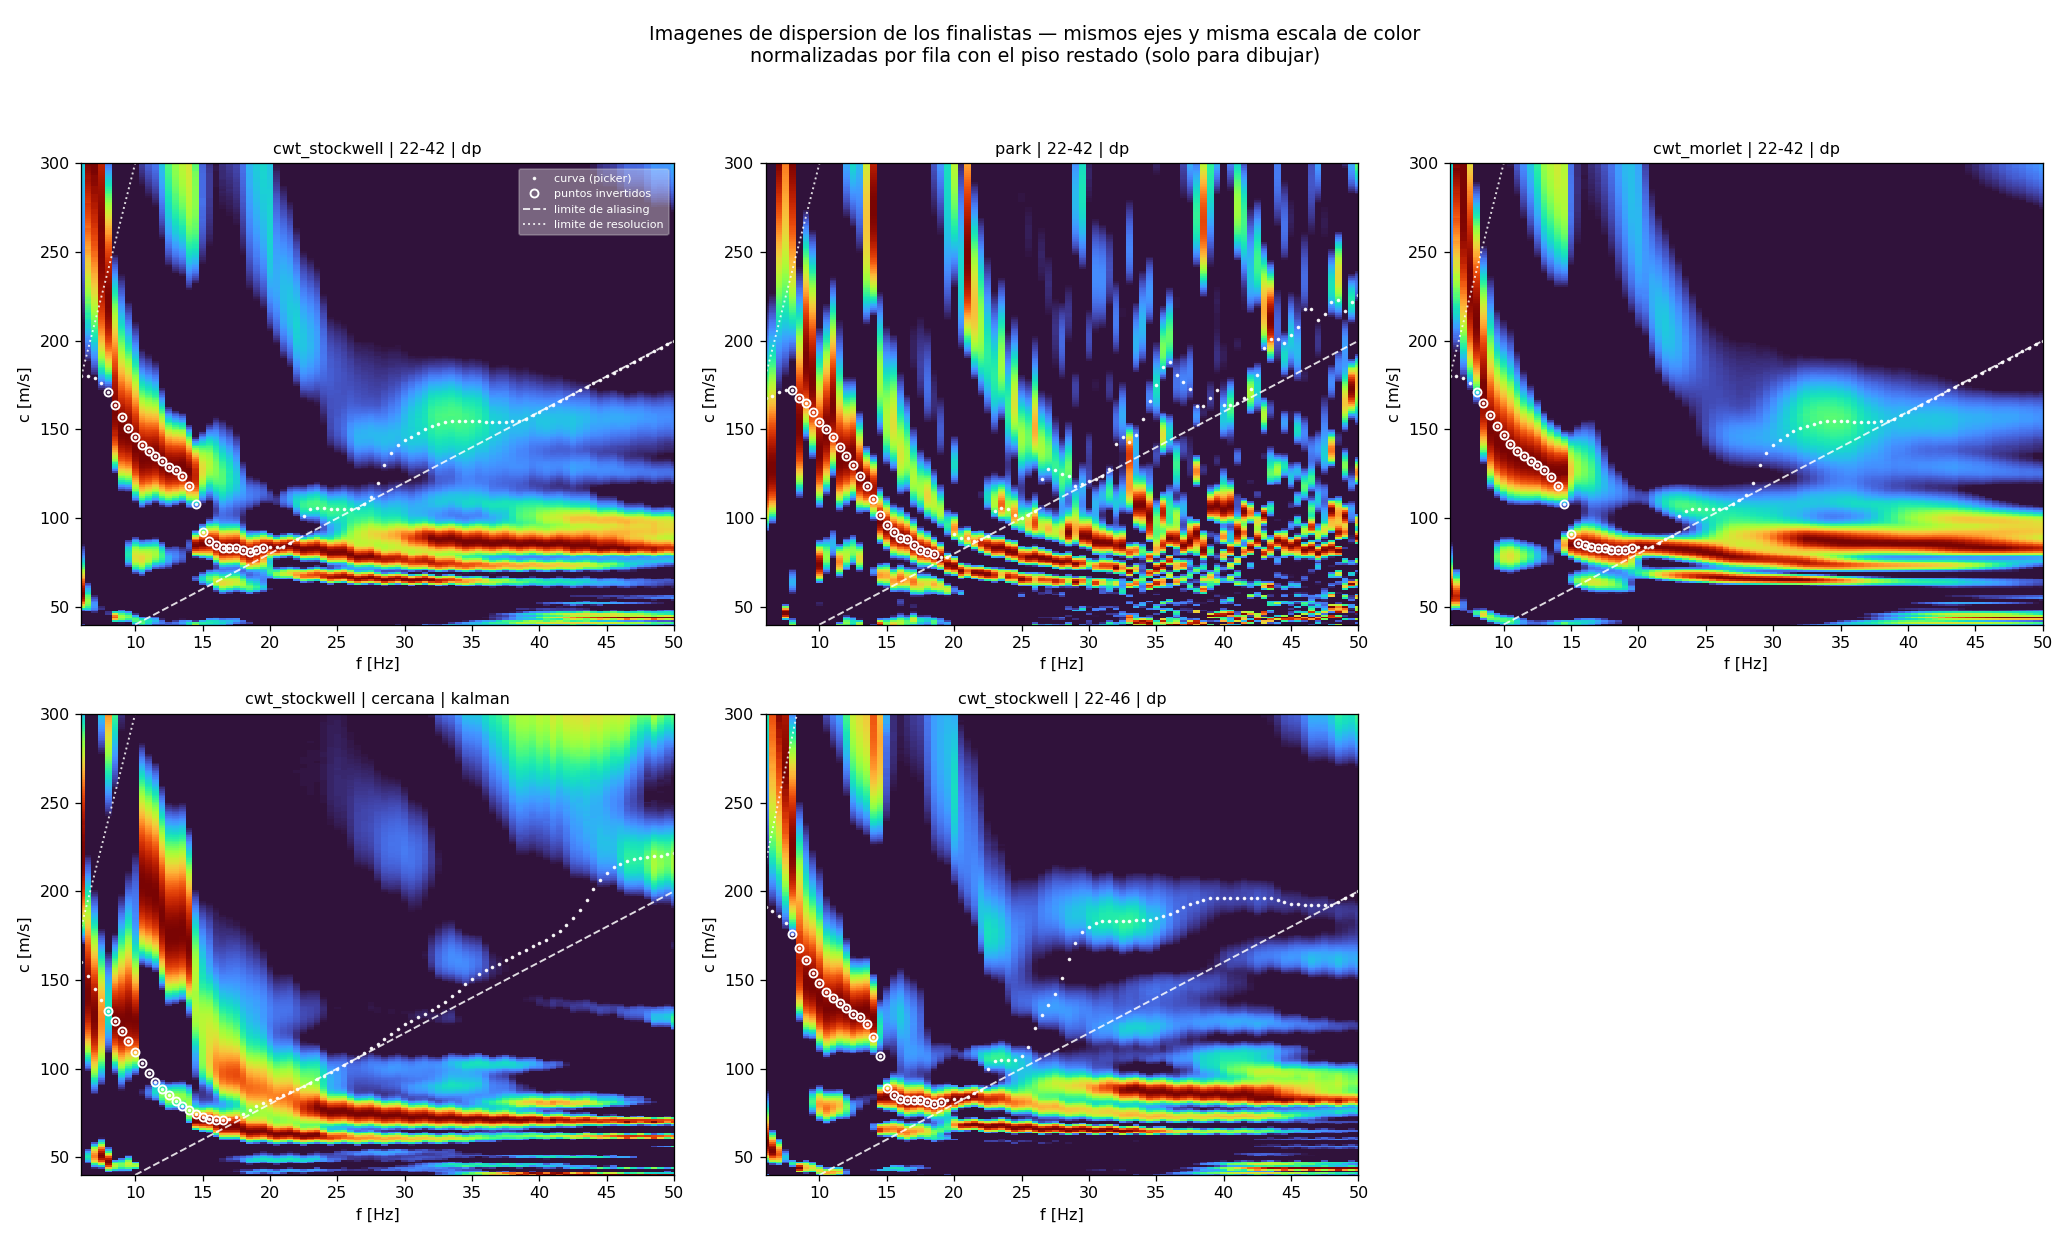
\includegraphics[width=\textwidth,keepaspectratio]{f_imagenes_dispersion.png}
\caption{Imágenes de dispersión en el plano frecuencia--velocidad de fase, normalizadas por frecuencia, de modo que los colores no comparan energía entre bandas. La línea dibujada es el límite de apertura del criterio de análisis adoptado. \revsolution{Fuente: elaboración propia a partir de los registros del proyecto.}}
\label{fig:dispersionimagenes}
\end{figure*}

\begin{figure*}[!tb]
\centering
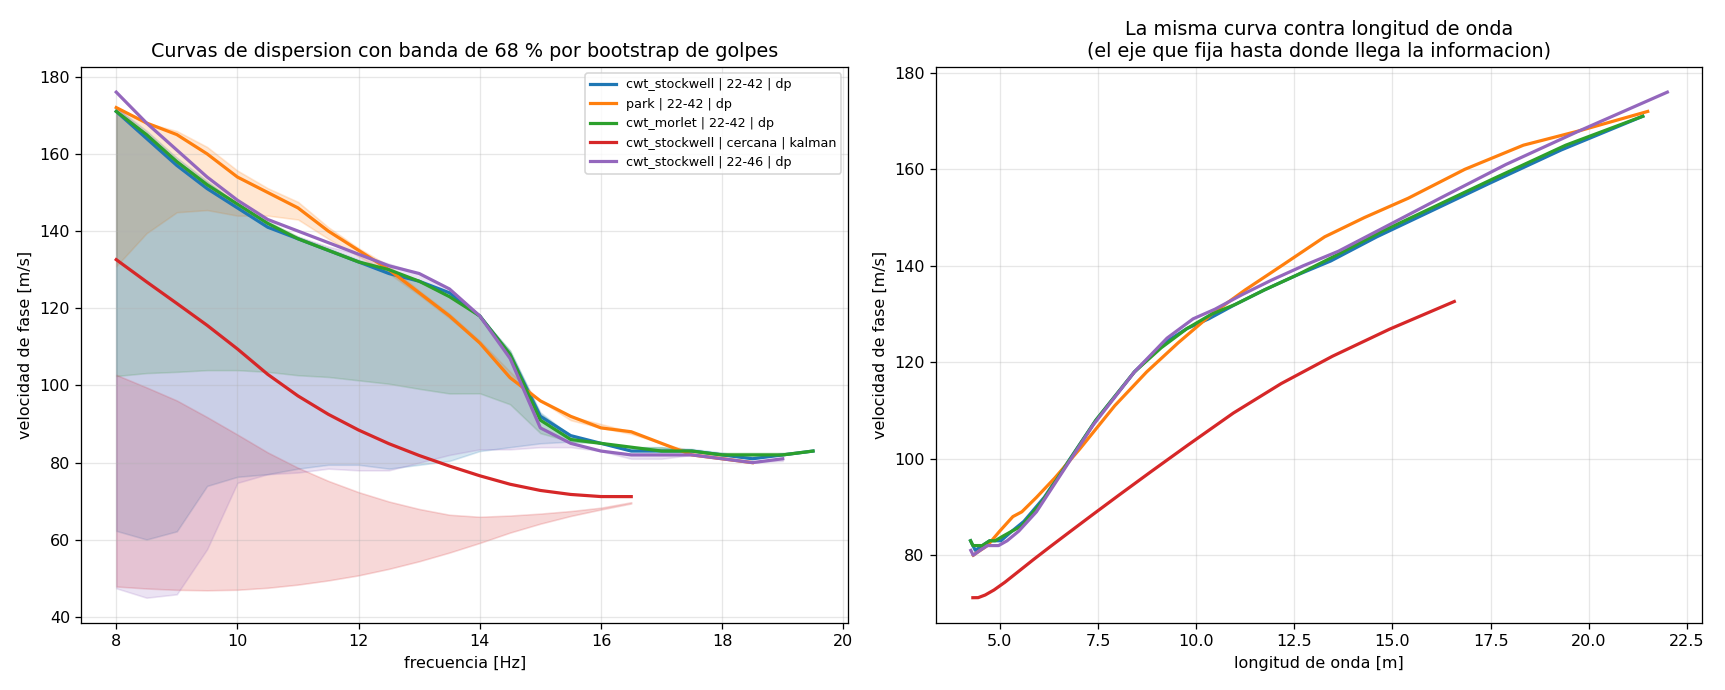
\includegraphics[width=\textwidth,keepaspectratio]{f_curvas_dispersion.png}
\caption{Curvas de dispersión extraídas y su longitud de onda asociada, con la banda de incertidumbre obtenida por remuestreo. La curva empleada para el modelo presentado es la del subarreglo de 22 a 42 m. \revsolution{Fuente: elaboración propia a partir de los registros del proyecto.}}
\label{fig:dispersioncurvas}
\end{figure*}

El análisis y la selección de subconjuntos de las mediciones permitieron identificar longitudes de onda de 20 a 22 m. Para el punto de 8 Hz y 172 m/s del subarreglo de 22 a 42 m,
\begin{equation}
\lambda_R=\frac{172}{8}=21{,}5\ \mathrm m,
\qquad z_{\mathrm{sop}}\simeq\frac{\lambda_R}{2}=10{,}75\ \mathrm m.
\label{eq:alcance-campo}
\end{equation}
La variable $z_{\mathrm{sop}}$ representa el alcance estimado con esta convención, que se informa como aproximadamente \textbf{10 a 11 m}.

\subsubsection{Perfil e incertidumbre de la inversión}

Se adoptó un modelo de tres capas para la ventana de 22 a 42 m. La elección se basó en 24 remuestreos por \revsolution{\emph{bootstrap} \citep{Efron1979}} y 5 semillas del optimizador, con 120 inversiones por configuración. Con tres capas, prácticamente toda la variabilidad del perfil provino del remuestreo de los datos; al incorporar una cuarta, cerca de la mitad provino del optimizador. El dato disponible no permitió sostener esa complejidad adicional.

El perfil presenta una velocidad de corte somera del orden de 78 m/s, una interfaz efectiva próxima a 2,4 m y velocidades cercanas a 178 m/s por debajo, dentro del alcance investigado. La interfaz representa el cambio de rigidez que reproduce la curva observada.

La inversión supone una velocidad de corte creciente con la profundidad y un coeficiente de Poisson adoptado. En pruebas sintéticas, la primera restricción ocultó una inversión de velocidad conocida; al retirarla del análisis de campo, el perfil quedó insuficientemente determinado. Variar el coeficiente de Poisson afectó poco a la velocidad somera y aumentó la incertidumbre en profundidad. Por ello, el perfil constituye una interpretación compatible con los datos, sin identificar de forma única los contactos geológicos. \revsolution{La no unicidad de la inversión de ondas superficiales está documentada por \citet{Foti2009}; las pruebas anteriores describen cómo se manifestó en los datos de este trabajo.} El alcance de 10 a 11 m tampoco permite calcular $V_{S,30}$.

\subsection{Sensibilidad al procesamiento y a la selección de posiciones}
\label{sec:sensibilidad-procesamiento}

Cambiar la transformada modificó la curva de dispersión en 2,28 m/s de mediana; cambiar el algoritmo de extracción, en 1,89 m/s. Al retirar las posiciones de 32 y 40 m, la diferencia cuadrática media fue de 29,76 m/s. En las comparaciones realizadas, la selección de posiciones tuvo mayor efecto que la elección de la transformada o del algoritmo de extracción. Este resultado respalda priorizar el control de la geometría y la calidad de los registros en la siguiente campaña.

\subsection{Contraste con sondeos eléctricos del predio}
\label{sec:contraste-sondeos}

\revsolution{El informe hidrogeológico de julio de 2023, elaborado por Víctor González \& Asoc. S.S., aporta un contraste de plausibilidad \citep{EstudioHidrogeologico2023}.} Sus sondeos eléctricos verticales se ubican en el mismo predio, a distancias del orden de 120, 258 y 340 m de la línea de adquisición, que no pueden precisarse por no haberse registrado las coordenadas de los extremos. El sondeo más próximo presenta interfaces eléctricas a 1,00, 2,06 y 4,15 m, de modo que la interfaz efectiva de 2,4 m obtenida por inversión cae dentro de un intervalo en el que el sondeo eléctrico también detecta contactos. La coincidencia debe leerse como compatibilidad en el intervalo de 2 a 4 m y de ninguna manera como un acuerdo de centímetros, tanto por la distancia entre emplazamientos como porque ambas técnicas miden propiedades distintas: la resistividad no mide rigidez y la velocidad de corte no mide contenido de humedad. El contraste sirve para verificar que el resultado no es físicamente inverosímil, no para validarlo.

% Mantener el título de la síntesis unido a su tabla de ancho completo.
\begin{table*}[!ht]
\subsection{Síntesis: qué está demostrado y qué no}
\label{sec:sintesis}

\centering
\footnotesize
\caption{Síntesis del estado de cada afirmación. \revsolution{Fuente: elaboración propia.}}
\begin{tabularx}{0.92\textwidth}{YYY}
\toprule
Afirmación & Estado & Base \\
\midrule
La plataforma adquiere de forma conjunta una referencia de impacto y la respuesta del receptor & Demostrado & 598 registros aceptados con referencia temporal \\
Los datos se almacenan, organizan y procesan mediante un flujo reproducible & Demostrado & Manifiesto, servidor de ingesta y análisis repetible \\
La transferencia PGA--ADC se identifica entre 0,21 Hz y 1,11 kHz & Demostrado para una unidad & 61 puntos; residuos del ajuste de 0,200 dB y 1,16° \\
La energía de campo se concentra entre 10 y 50 Hz; la curva utilizada parte de unos 8 Hz & Medido; condicionado por el procesamiento & Métricas sobre 265 golpes en 15 distancias y curva de dispersión \\
Un arreglo sintetizado de 21 posiciones permite obtener imagen y curva de dispersión & Demostrado & Procesamiento de la campaña \\
El soporte de investigación es de aproximadamente 10 a 11 m & Preliminar & Longitud de onda soportada y convención $z\approx\lambda/2$ \\
El perfil de tres capas describe el sitio & Preliminar & 120 inversiones por configuración; sujeto a monotonía y a $\nu$ supuesto \\
La interfaz de 2,4 m corresponde a un contacto geológico & No afirmado & Es una interfaz efectiva del modelo \\
Adquisición simultánea con varios nodos GEO completos & No demostrado & Un solo nodo GEO íntegro operativo por registro \\
Coordinación de arranque con tres nodos simultáneos & Demostrado funcionalmente & Ensayo de laboratorio sobre los módulos de radio \\
Sincronización entre nodos dentro de unos 670 µs & No demostrado & Sin registros comparables entre placas completas \\
Ruido del instrumento & No medido & Caracterización pendiente \\
Extensión hacia capas más profundas y cálculo de $V_{S,30}$ & Trabajo futuro & El perfil actual tiene soporte hasta unos 10--11 m \\
\bottomrule
\end{tabularx}
\end{table*}

\section{Limitaciones y trabajos futuros}
\label{sec:limitaciones}

\textbf{Ruido del instrumento.} Se propone caracterizar el ruido para las configuraciones de ganancia y rango utilizadas.

\textbf{Operación multicanal.} Se completará la revisión de placa y la operación conjunta de varios nodos GEO, verificando la dispersión de ganancia y fase y la sincronización respecto de la tolerancia de unos 670 $\mu$s.

\textbf{Geometría y protocolo.} Se plantea registrar coordenadas y azimut, mantener una referencia de impacto y ensayar una mayor apertura efectiva para extender la caracterización por debajo de los 8 Hz actuales hacia capas más profundas.

\textbf{Fuente y extensión de la banda de excitación.} Se propone ensayar una fuente de impactos periódicos cuyo período pueda variarse. Para un período $T$, la frecuencia fundamental $f_p$ y sus armónicos $f_k$ cumplen
\begin{equation}
f_p=\frac{1}{T},\qquad f_k=\frac{k}{T},
\quad k=1,2,\ldots
\label{eq:fuente-periodica}
\end{equation}
donde $k$ es el orden del armónico \revsolution{\citep[cap.~13]{Smith1997}}. Al variar el período entre ensayos se desplazan la fundamental y sus armónicos. Se evaluará si esta excitación permite obtener registros coherentes a frecuencias menores.


\FloatBarrier
\bibliographystyle{apalike}
{\footnotesize
\bibliography{referencias}}

\end{document}
